%%%%%%%%%%%%%%%%%%%%%%%%%%%%%%%%%%%%%%%%%
% Beamer Presentation
% LaTeX Template
% Version 1.0 (10/11/12)
%
% This template has been downloaded from:
% http://www.LaTeXTemplates.com
%
% License:
% CC BY-NC-SA 3.0 (http://creativecommons.org/licenses/by-nc-sa/3.0/)
%
%%%%%%%%%%%%%%%%%%%%%%%%%%%%%%%%%%%%%%%%%

%----------------------------------------------------------------------------------------
%	PACKAGES AND THEMES
%----------------------------------------------------------------------------------------

\documentclass[aspectratio-169]{beamer}

\mode<presentation> {

% The Beamer class comes with a number of default slide themes
% which change the colors and layouts of slides. Below this is a list
% of all the themes, uncomment each in turn to see what they look like.

%\usetheme{default}
%\usetheme{AnnArbor}
%\usetheme{Antibes}
%\usetheme{Bergen}
%\usetheme{Berkeley}
%\usetheme{Berlin}
%\usetheme{Boadilla}
%\usetheme{CambridgeUS}
%\usetheme{Copenhagen}
%\usetheme{Darmstadt}
%\usetheme{Dresden}
%\usetheme{Frankfurt}
%\usetheme{Goettingen}
%\usetheme{Hannover}
%\usetheme{Ilmenau}
%\usetheme{JuanLesPins}
%\usetheme{Luebeck}
\usetheme{Madrid}
%\usetheme{Malmoe}
%\usetheme{Marburg}
%\usetheme{Montpellier}
%\usetheme{PaloAlto}
%\usetheme{Pittsburgh}
%\usetheme{Rochester}
%\usetheme{Singapore}
%\usetheme{Szeged}
%\usetheme{Warsaw}

% As well as themes, the Beamer class has a number of color themes
% for any slide theme. Uncomment each of these in turn to see how it
% changes the colors of your current slide theme.

%\usecolortheme{albatross}
%\usecolortheme{beaver}
%\usecolortheme{beetle}
%\usecolortheme{crane}
%\usecolortheme{dolphin}
%\usecolortheme{dove}
%\usecolortheme{fly}
%\usecolortheme{lily}
%\usecolortheme{orchid}
%\usecolortheme{rose}
%\usecolortheme{seagull}
%\usecolortheme{seahorse}
%\usecolortheme{whale}
%\usecolortheme{wolverine}

%\setbeamertemplate{footline} % To remove the footer line in all slides uncomment this line
%\setbeamertemplate{footline}[page number] % To replace the footer line in all slides with a simple slide count uncomment this line

%\setbeamertemplate{navigation symbols}{} % To remove the navigation symbols from the bottom of all slides uncomment this line
}

\usepackage{graphicx} % Allows including images
\usepackage{booktabs} % Allows the use of \toprule, \midrule and \bottomrule in tables

%----------------------------------------------------------------------------------------
%	TITLE PAGE
%----------------------------------------------------------------------------------------

\title[]{Interaction of Charged Particles with Different Materials} % The short title appears at the bottom of every slide, the full title is only on the title page

\author{Sharod Roy} % Your name
\institute[ICR] % Your institution as it will appear on the bottom of every slide, may be shorthand to save space
{
Institute for Computing in Research \\ % Your institution for the title page
\medskip
}
\date{\today} % Date, can be changed to a custom date

\begin{document}

\begin{frame}
\titlepage % Print the title page as the first slide
\end{frame}

%----------------------------------------------------------------------------------------
%	PRESENTATION SLIDES
%----------------------------------------------------------------------------------------

%------------------------------------------------

\begin{frame}
\frametitle{What is a Particle?}
\begin{itemize}
\item small collection of matter
\item described by mass, charge, and type
\end{itemize}
\begin{center}
    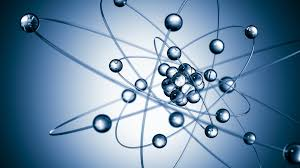
\includegraphics[width=0.5\textwidth]{images.jpeg}
    \footnote{[https://www.innovationnewsnetwork.com/wp-content/uploads/2021/02/Success-in-particle-physics-1536x864.jpg]}
\end{center}
\end{frame}

%------------------------------------------------

\begin{frame}
\frametitle{Project Description}
\begin{itemize}
    \item How do particles interact with different materials?
    \item Parameters of Experiment:
    \begin{itemize}
        \item Particles: p, e-, mu+, mu- 
        \item Materials: Aluminum (Al), Gold (Au), Iron (Fe), Plastic, Uranium (U)
        \item Energy Levels: 1,000 MeV, 10,000 MeV, 100,000 MeV
    \end{itemize}

\end{itemize}
\end{frame}

%------------------------------------------------
\begin{frame}
\frametitle{Geant4 Software}

\begin{itemize}
    \item Stands for GEometry ANd Tracking
    \item Uses Monte Carlo methods
    \item Simulation of the passage of particles through matter
    \item Written in C++
\end{itemize}

% Image layout
\begin{figure}
    \centering
    \begin{minipage}[b]{0.4\textwidth}
        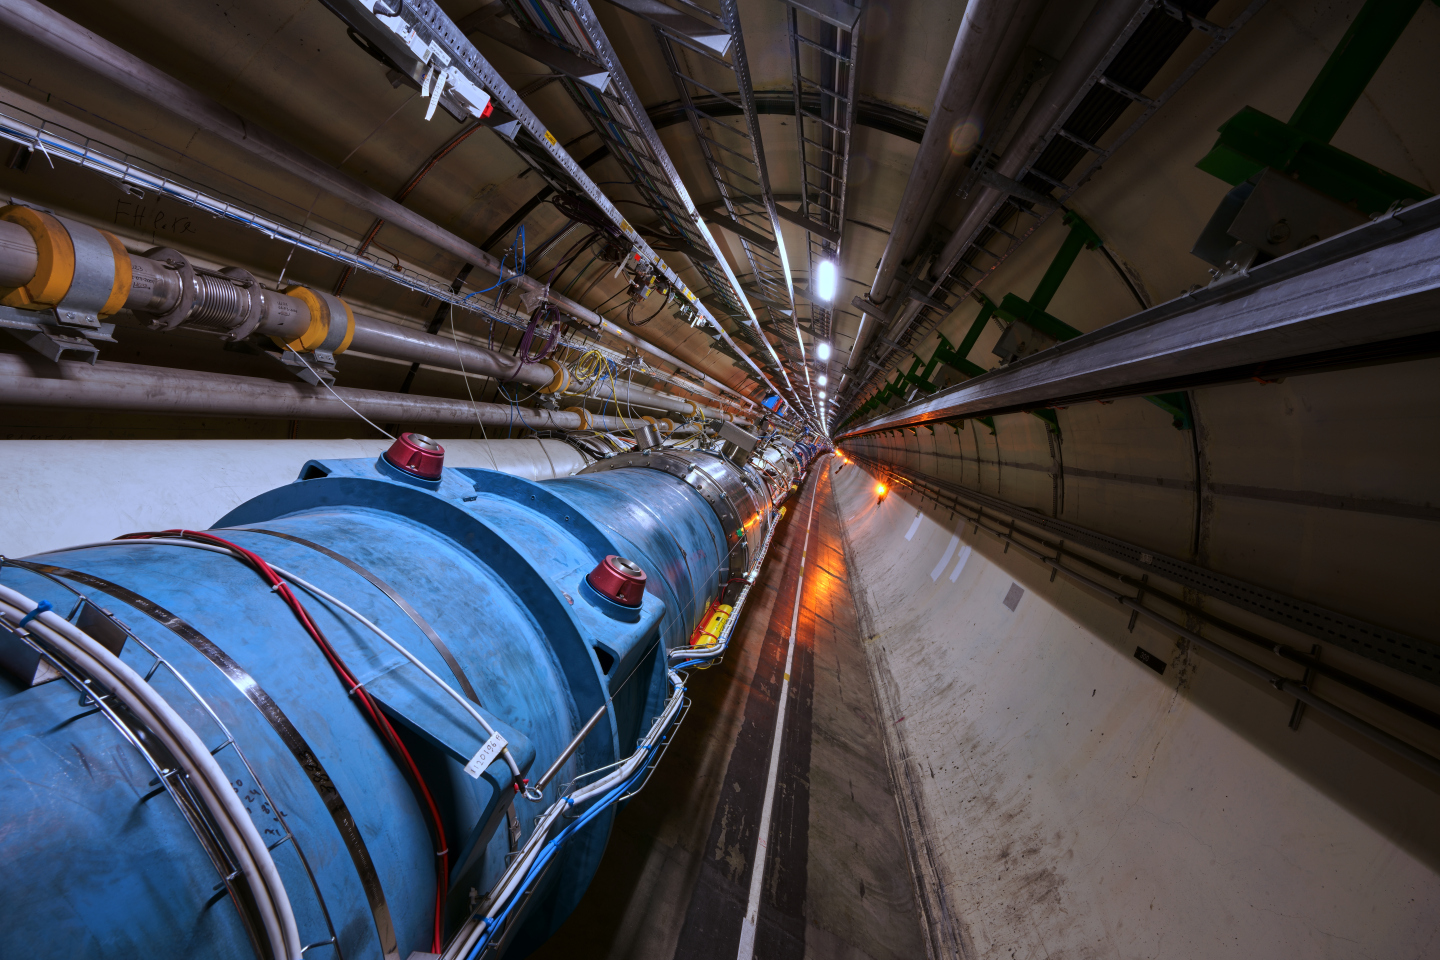
\includegraphics[width=\textwidth]{lhc.jpg}
        \caption{LHC Tunnel}
    \end{minipage}
    \hfill
    \begin{minipage}[b]{0.4\textwidth}
        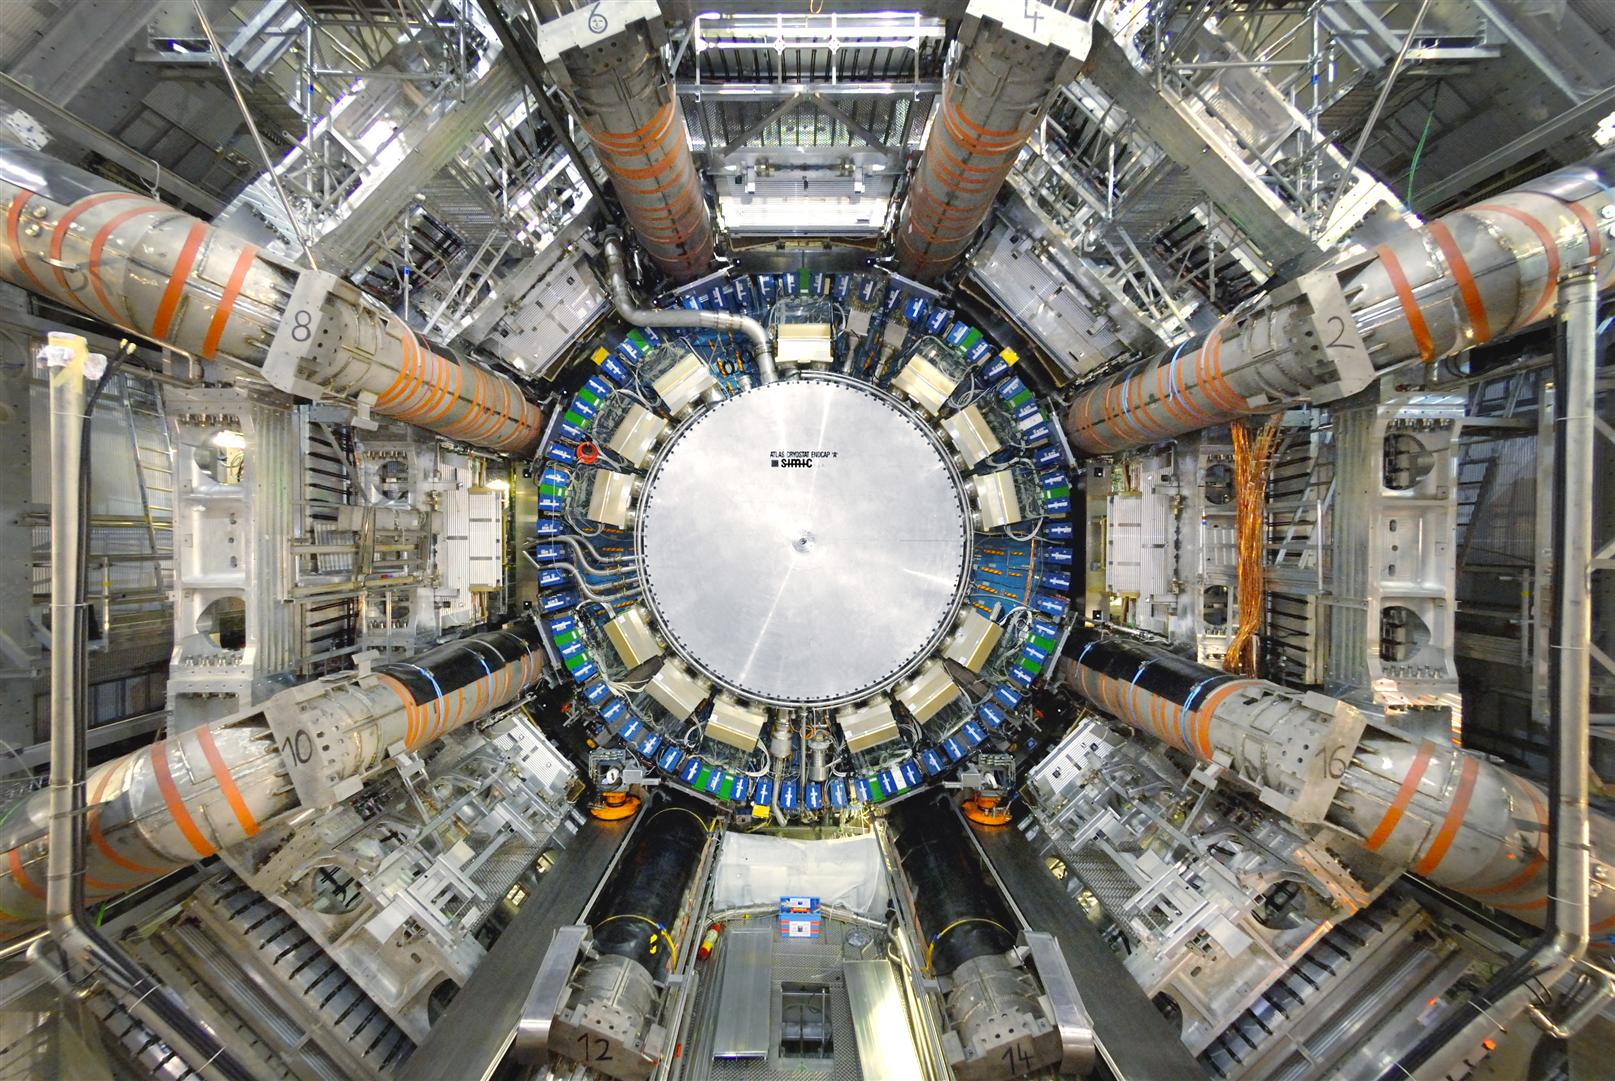
\includegraphics[width=\textwidth]{atlas.jpg}
        \caption{ATLAS Detector}
    \end{minipage}
    \hfill
    \begin{minipage}[b]{0.15\textwidth}
        
\includegraphics[width=\textwidth]{ISO_C++_Logo.svg.png}
    \end{minipage}
\end{figure}
\end{frame}

%------------------------------------------------

\begin{frame}
\frametitle{Visualization of Build}
\begin{itemize}
    \item 
    \begin{minipage}{0.85\textwidth}
        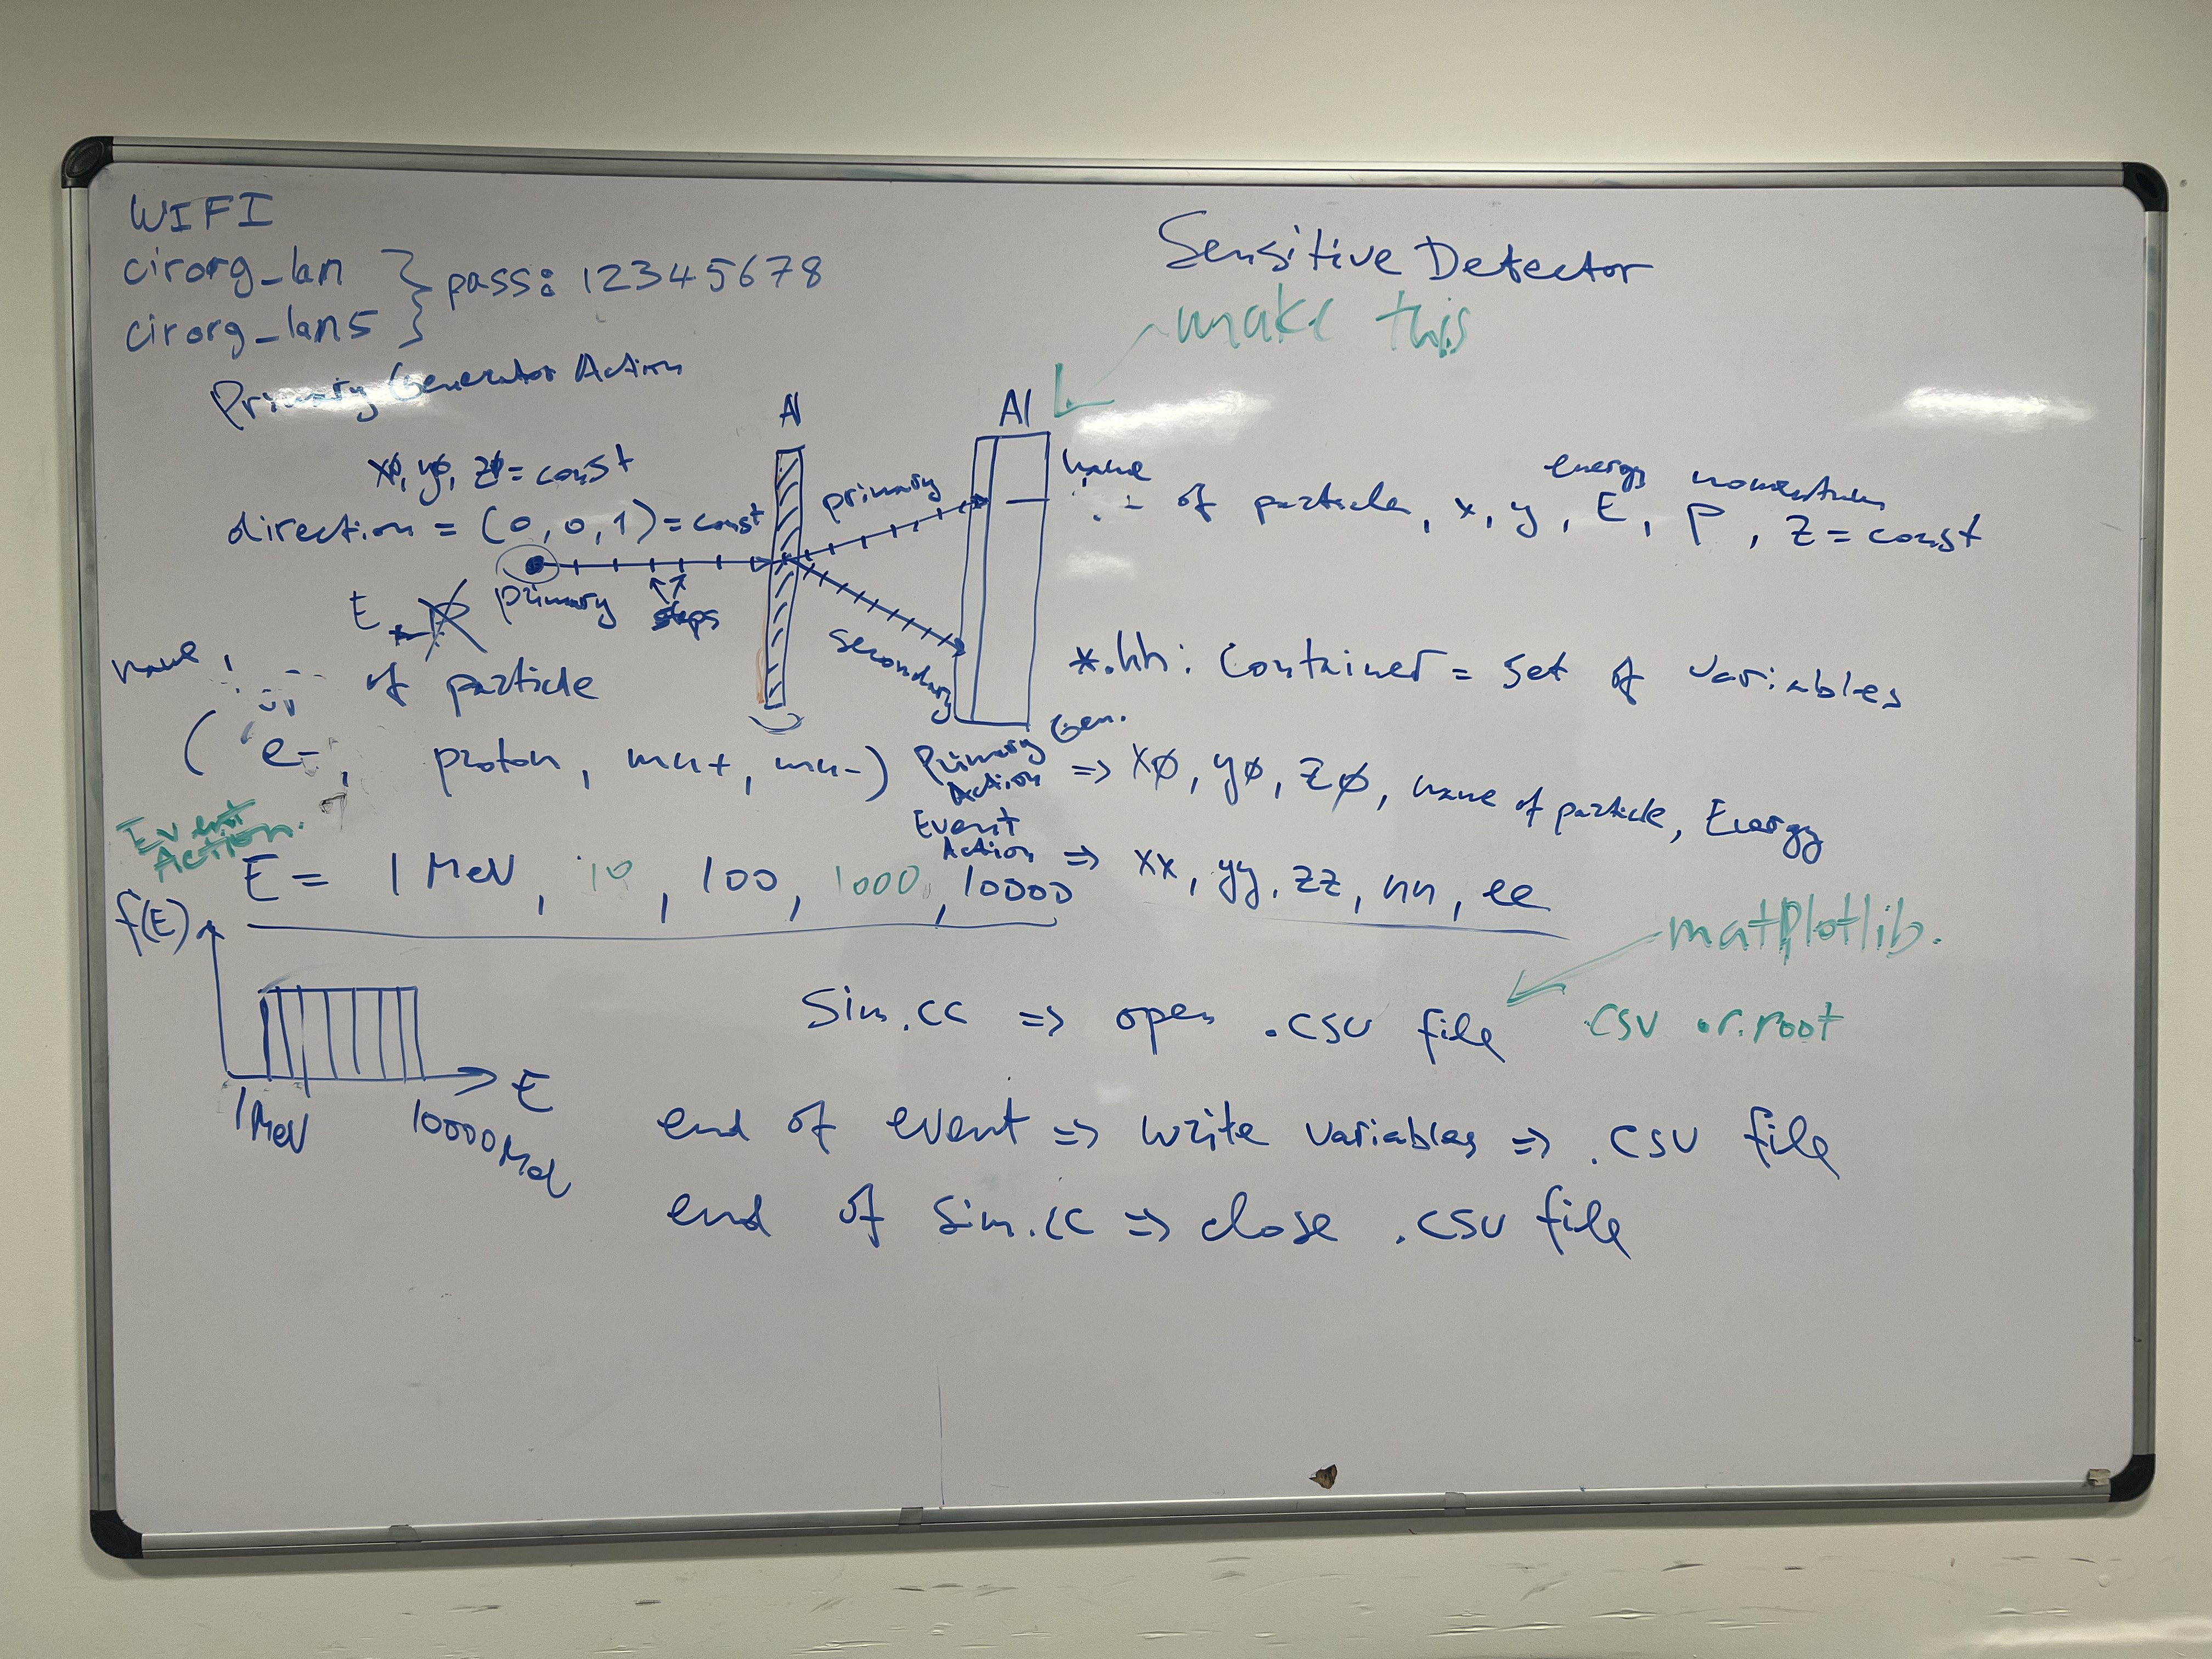
\includegraphics[width=\textwidth]{IMG_5434.jpg}
    \end{minipage}
\end{itemize}
\end{frame}

%------------------------------------------------

\begin{frame}
\frametitle{Code for Build}
\begin{itemize}
    \item 
    \begin{minipage}{0.85\textwidth}
        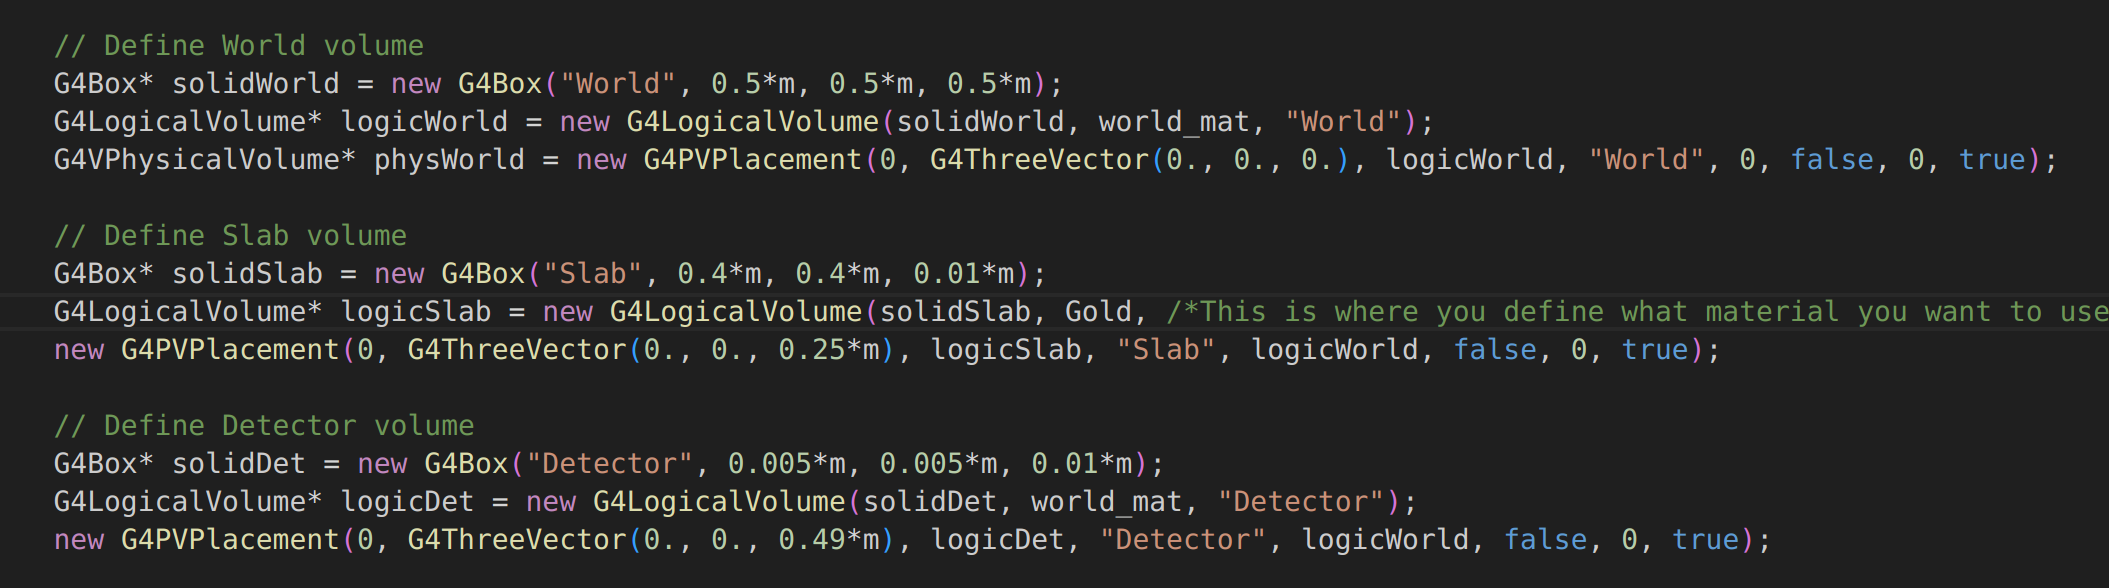
\includegraphics[width=\textwidth]{vis-code.png}
    \end{minipage}
    \hfill
    \begin{minipage}{0.85\textwidth}
        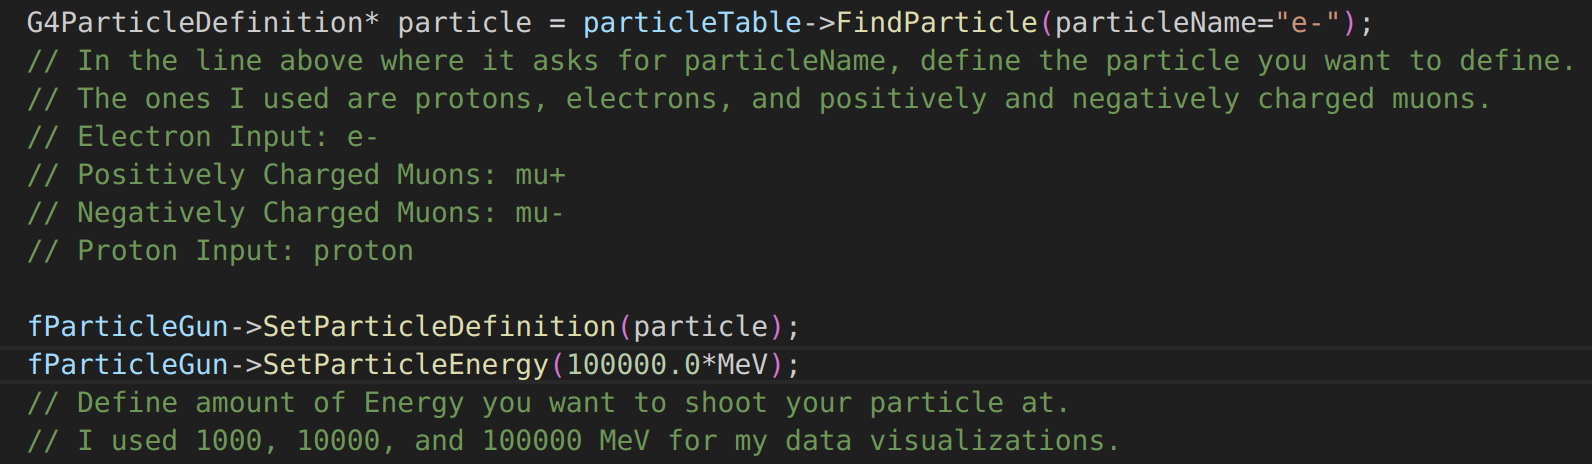
\includegraphics[width=\textwidth]{code.png}
    \end{minipage}
\end{itemize}
\end{frame}

%------------------------------------------------

\begin{frame}
\frametitle{Sketch}
\begin{itemize}
    \item 
    \begin{minipage}{0.65\textwidth}
        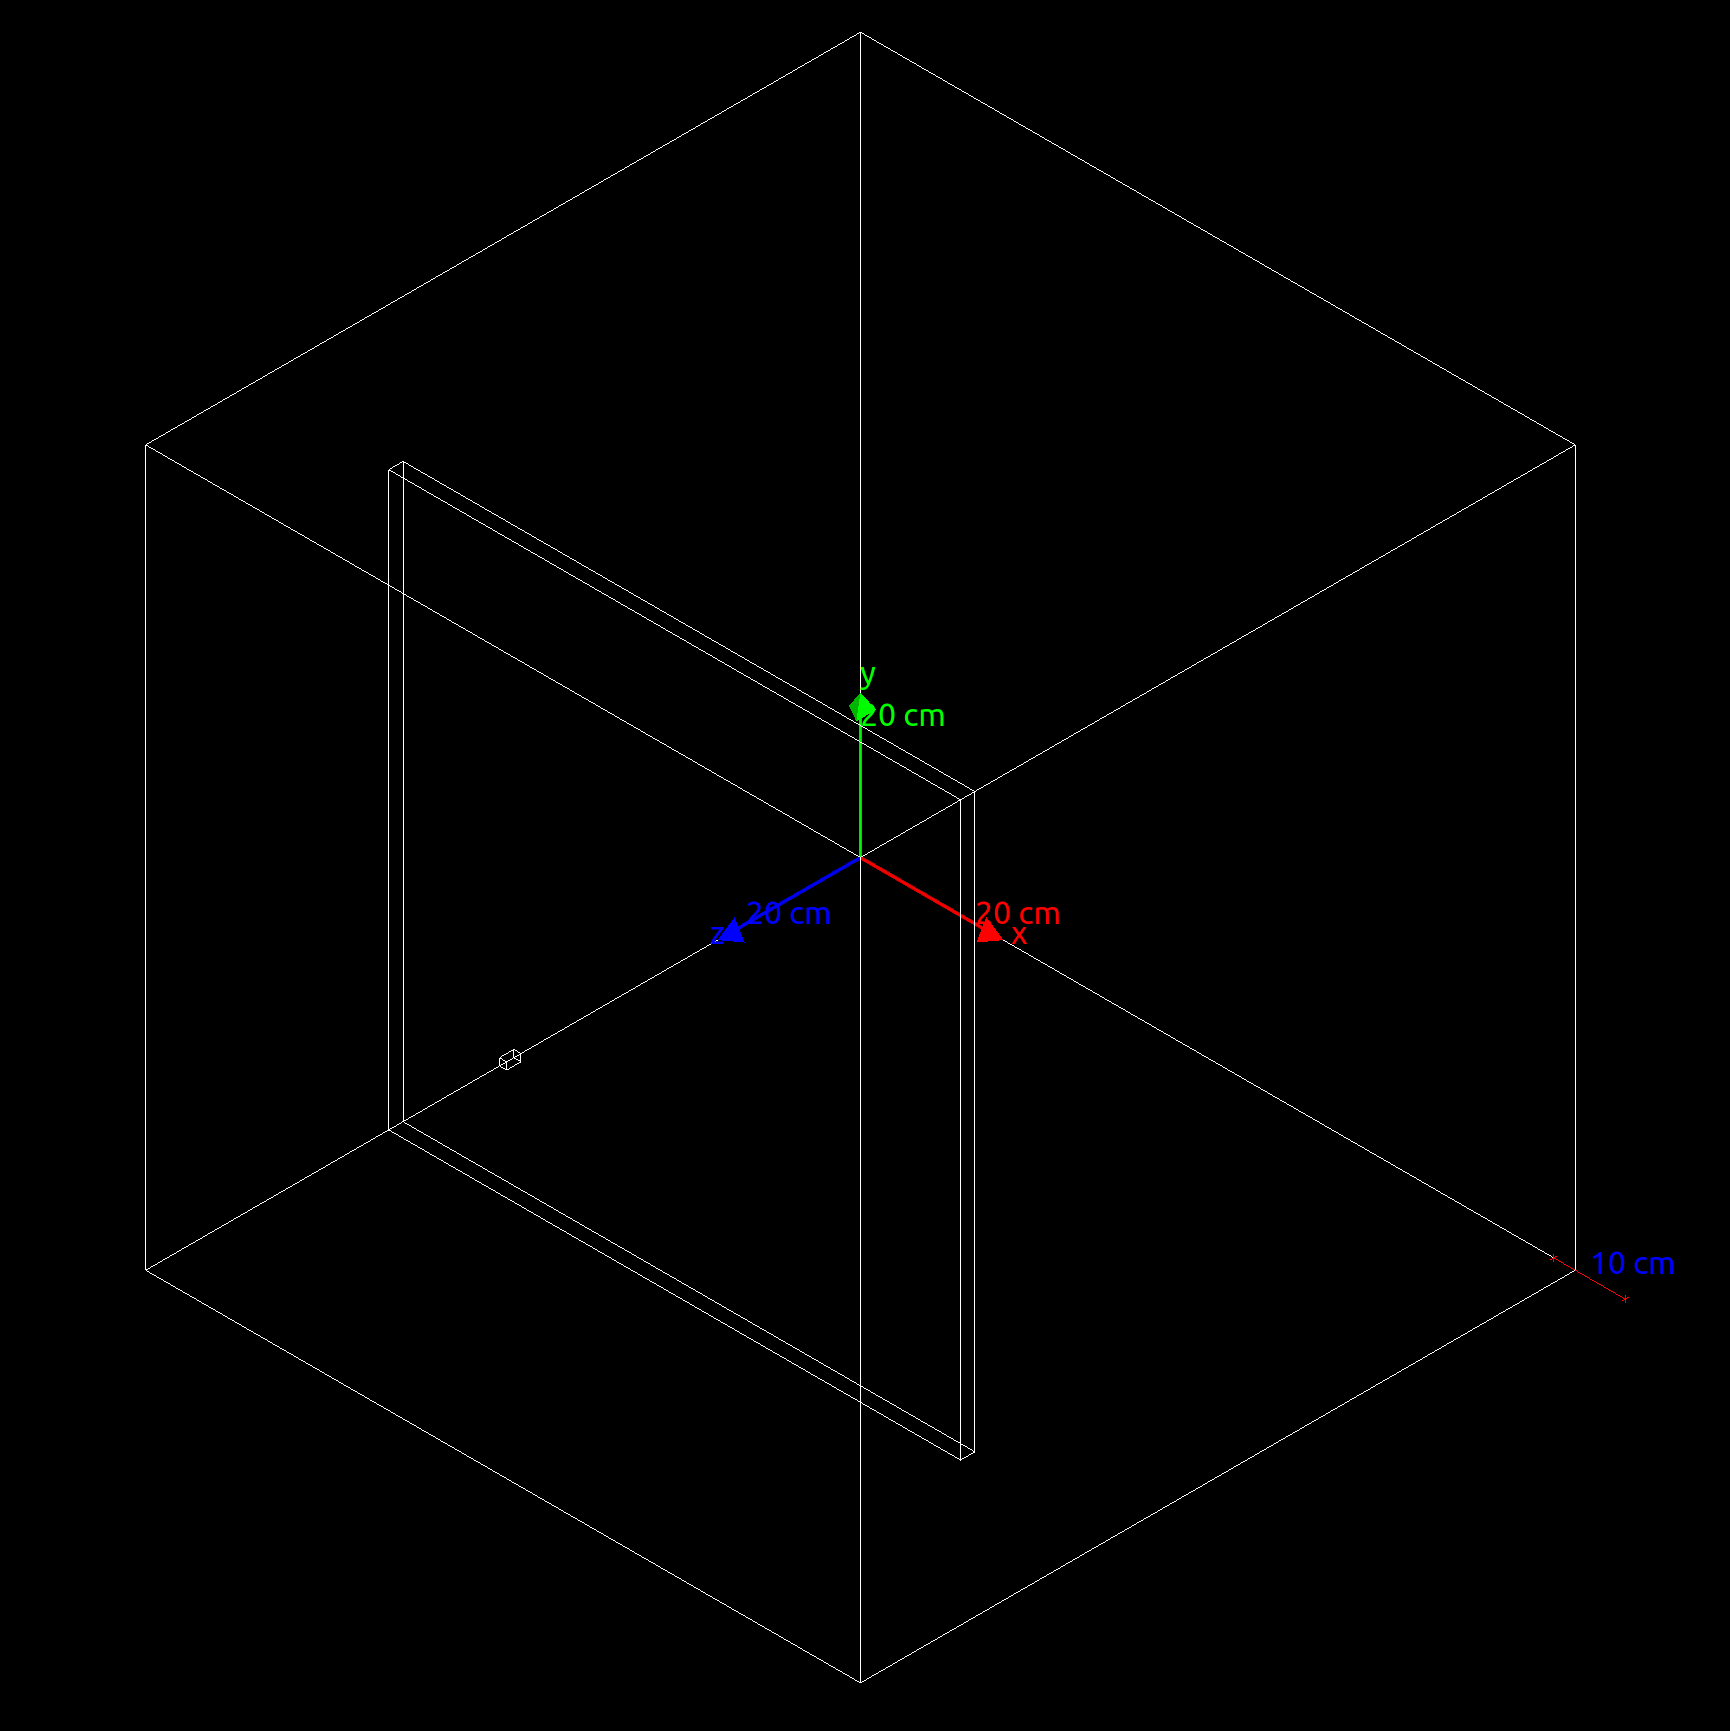
\includegraphics[width=\textwidth]{vis.png}
    \end{minipage}
\end{itemize}
\end{frame}

%------------------------------------------------

\begin{frame}
\frametitle{Output}
\begin{itemize}
    \item 
    \begin{minipage}{0.5\textwidth}
        \begin{figure}
            \centering
            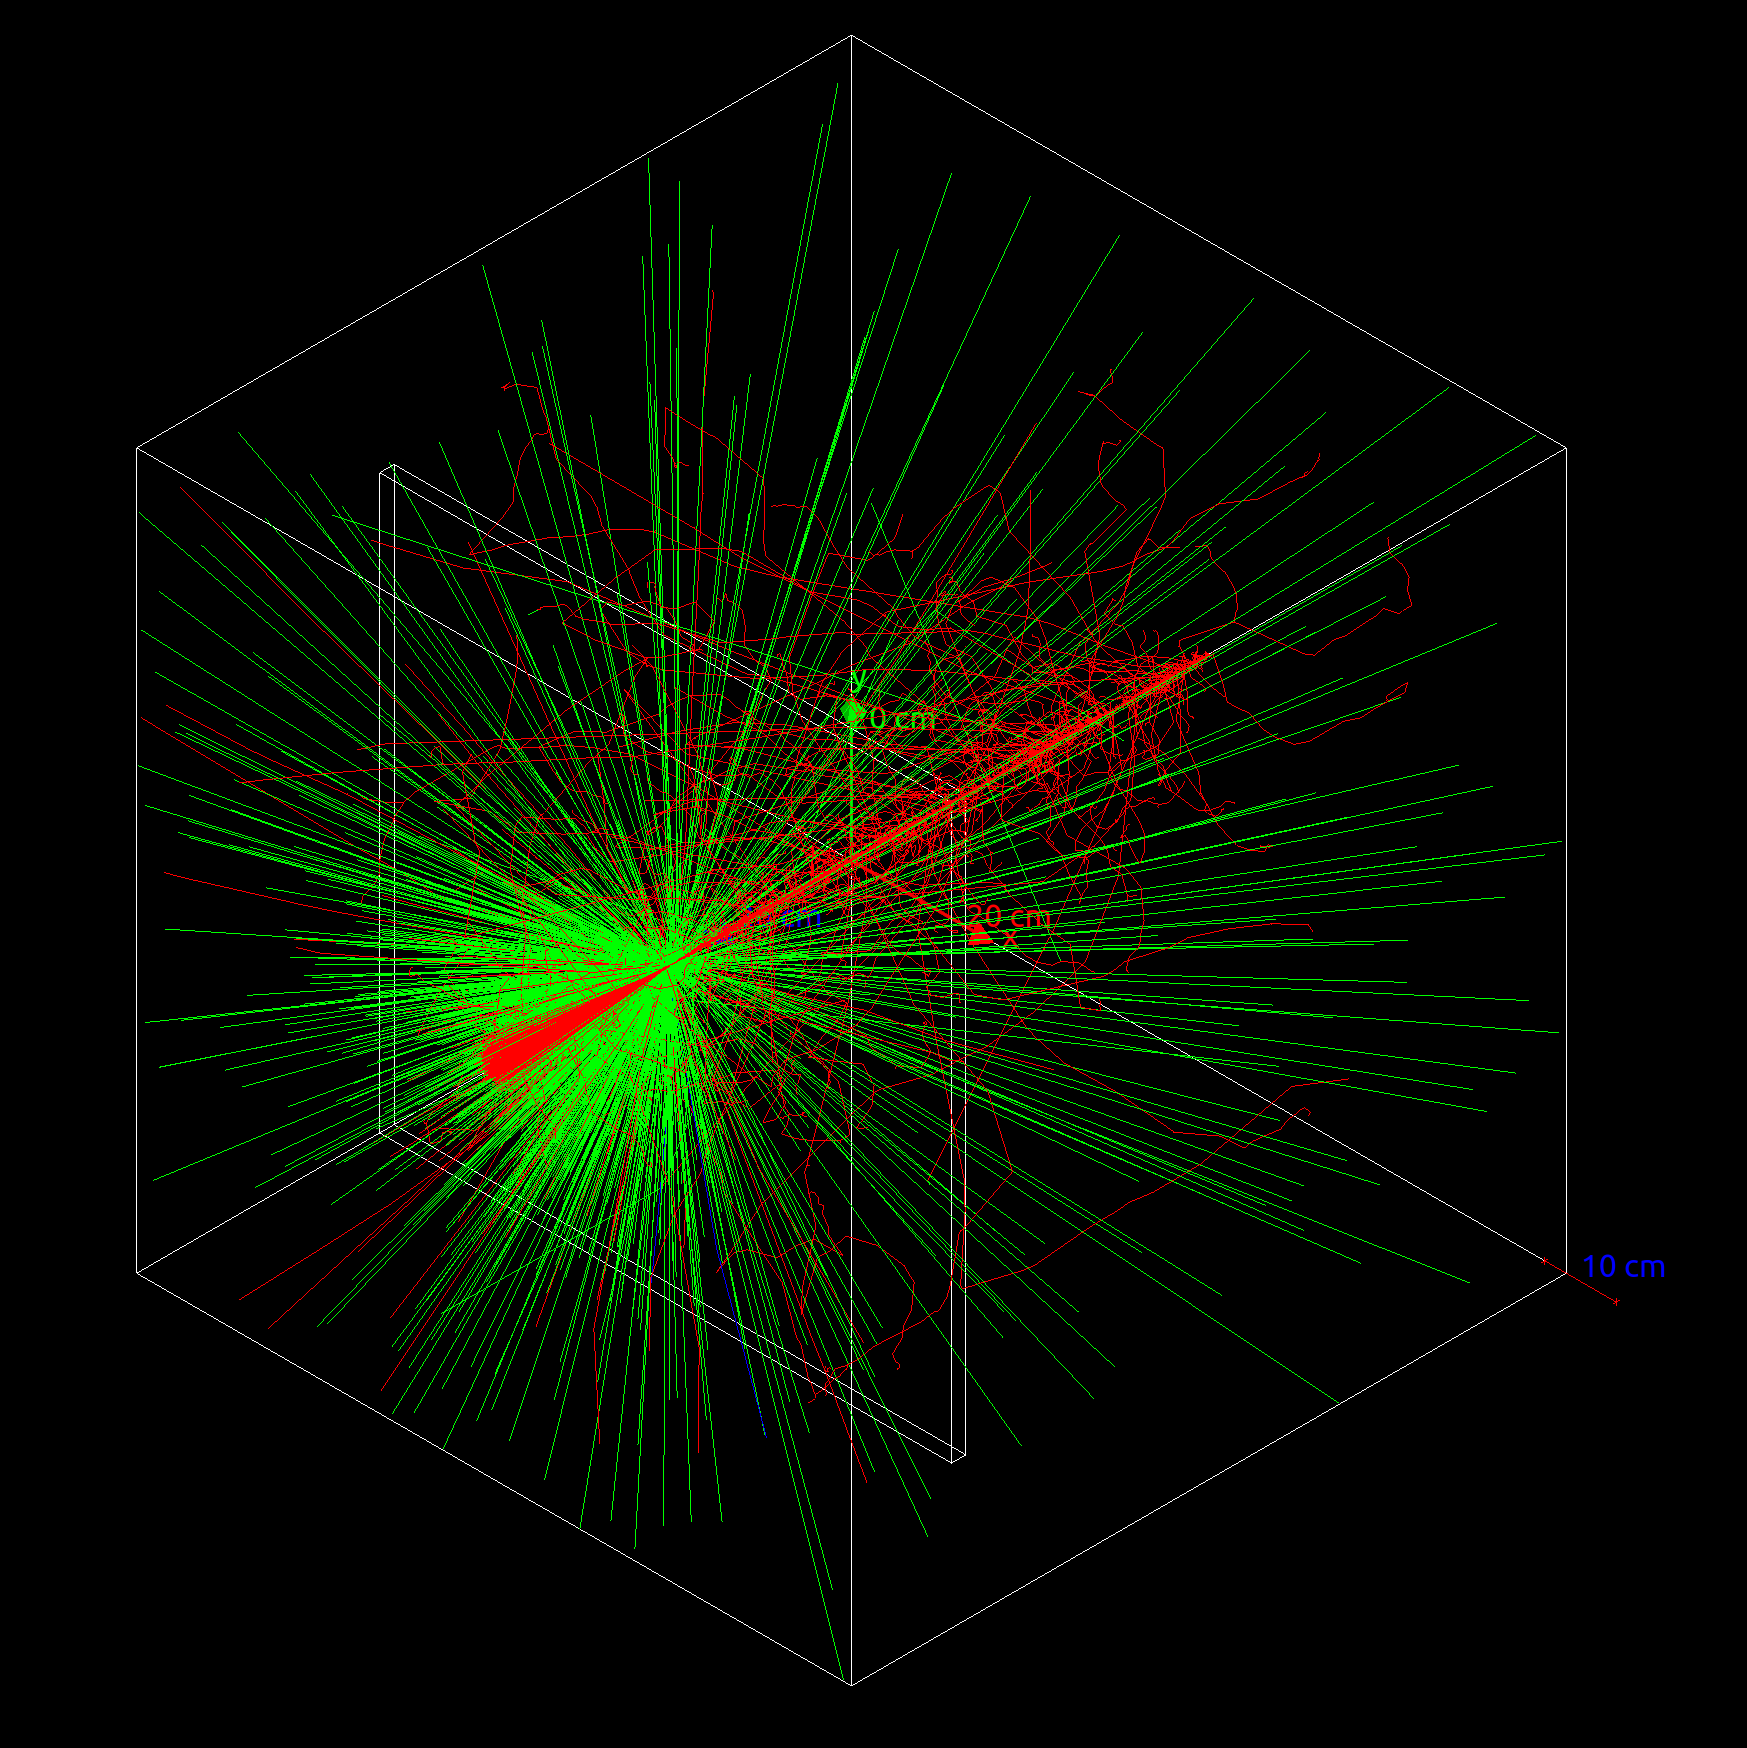
\includegraphics[width=\textwidth]{output.png}
            \caption{This is an example visualization of 100,000 negatively charged muons being shot at 1,000 MeV at a Gold Slab.}
        \end{figure}
    \end{minipage}
\end{itemize}
\end{frame}

%------------------------------------------------
\begin{frame}
\frametitle{Data Visualization}
\begin{itemize}
\item Data was given in .csv file
\item Three Types of Graphs:
    \begin{itemize}
    \item Position X vs. Position Y
    \item \# of Particles vs. Radius of Detector Plane
    \item Momentum vs. f(Momentum)
    \end{itemize}
\end{itemize}
\end{frame}

%------------------------------------------------

\begin{frame}
\frametitle{Proton (p) - PositionX vs PositionY}
\begin{itemize}
    \item 
    \begin{minipage}{0.5\textwidth}
        \begin{figure}
            \centering
            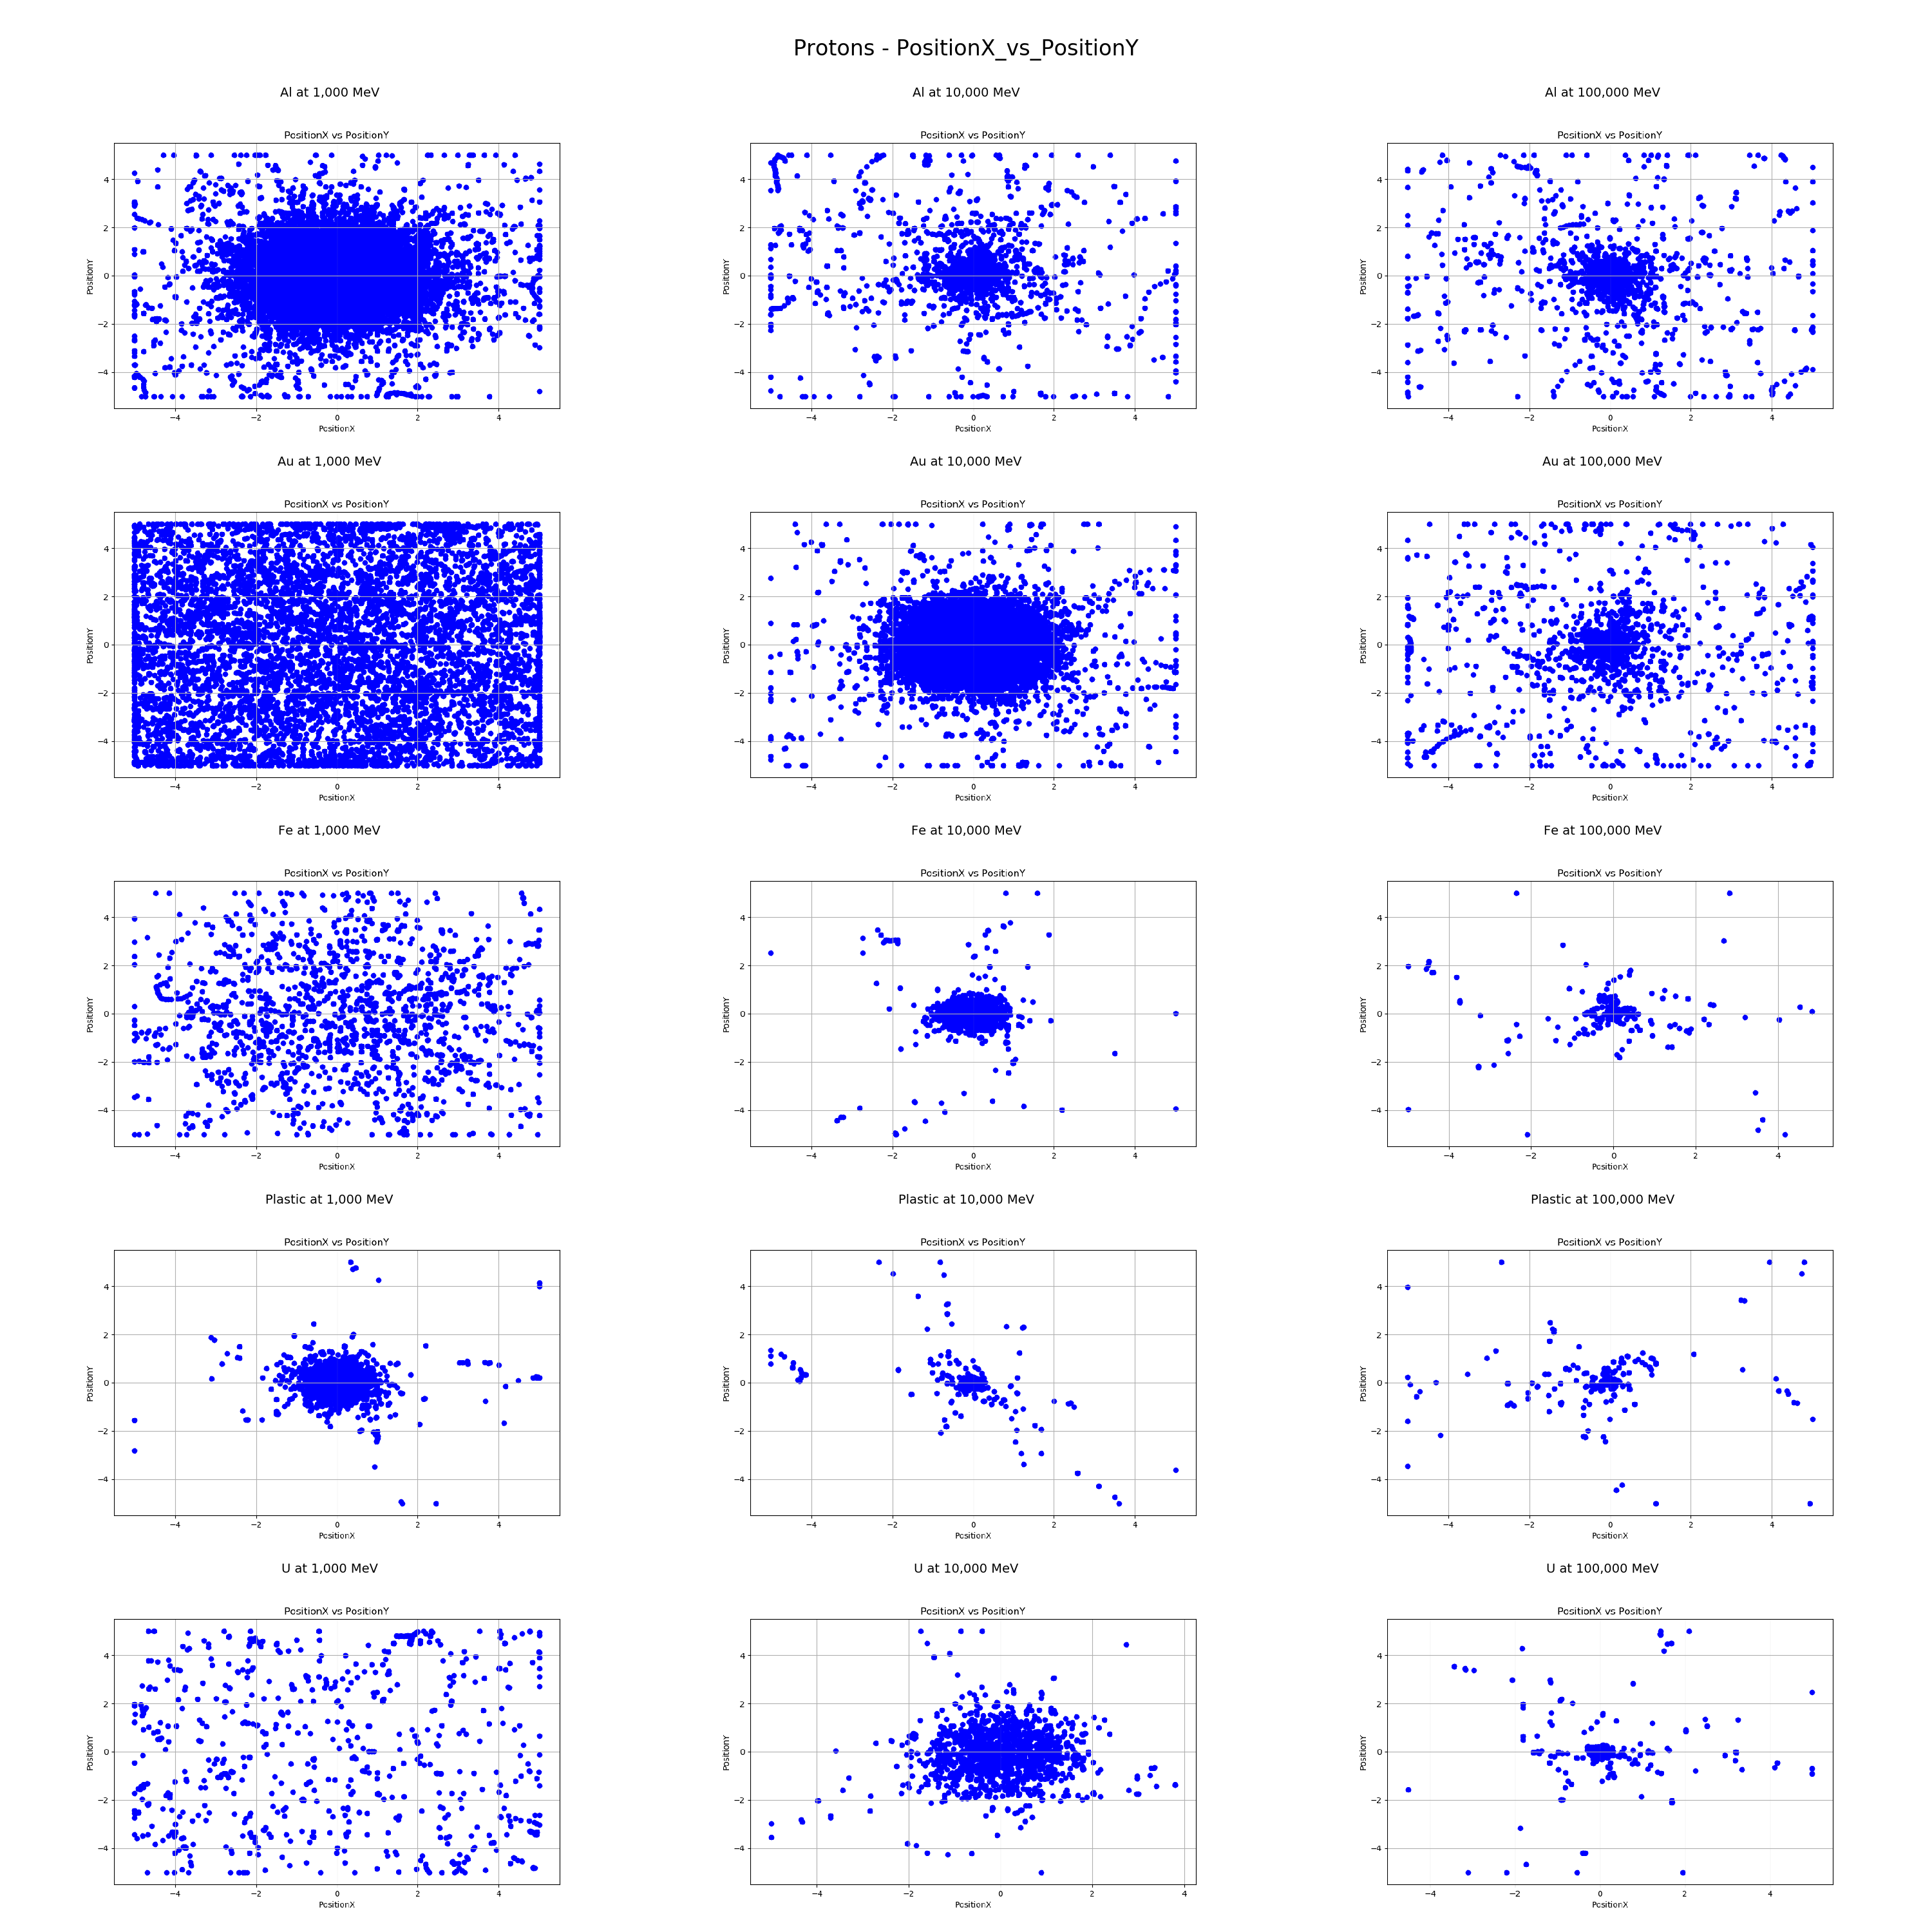
\includegraphics[width=\textwidth]{Combined Plots/PositionX_vs_PositionY_p.png}
            \footnotesize{Starts off as scattered everywhere and then concentrates into one point.}
        \end{figure}
    \end{minipage}
\end{itemize}
\end{frame}

%------------------------------------------------

\begin{frame}
\frametitle{Electron (e-) - PositionX vs PositionY}
\begin{itemize}
    \item 
    \begin{minipage}{0.5\textwidth}
        \begin{figure}
            \centering
            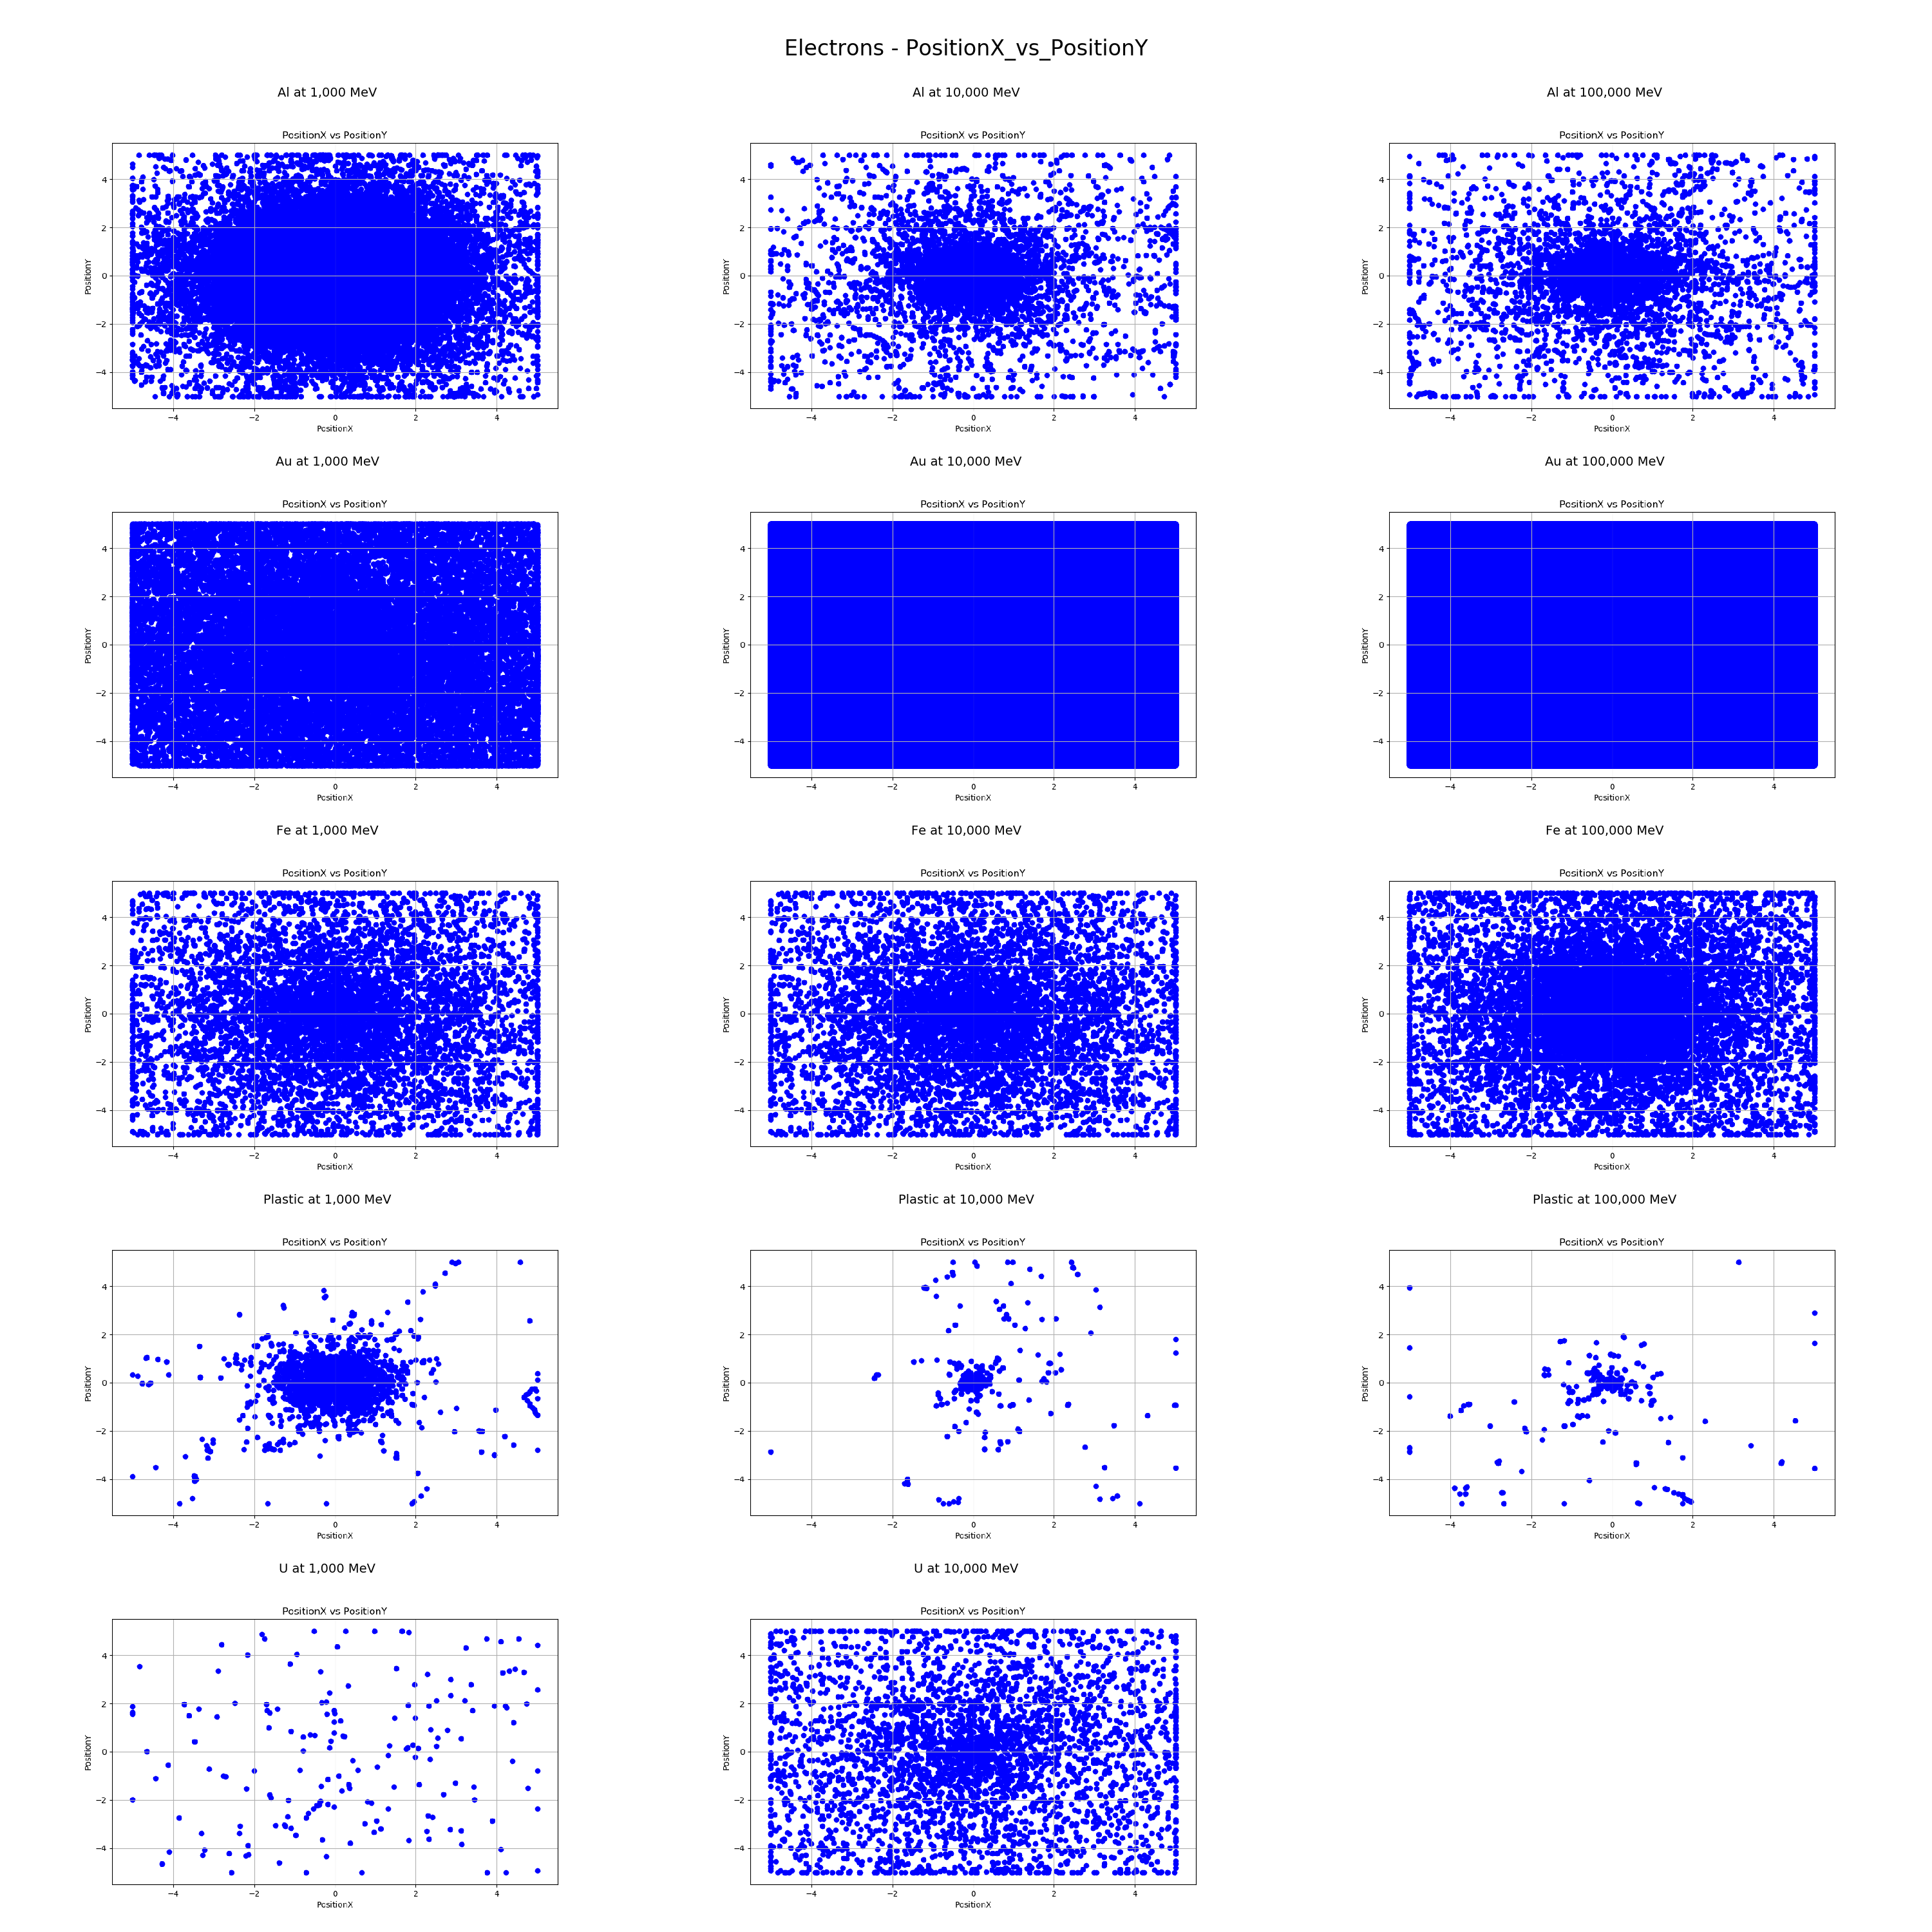
\includegraphics[width=\textwidth]{Combined Plots/PositionX_vs_PositionY_e-.png}
            \footnotesize{Electrons just scatter everywhere.}
        \end{figure}
    \end{minipage}
\end{itemize}
\end{frame}

%------------------------------------------------

\begin{frame}
\frametitle{Positively Charged Muons (mu+) - PositionX vs PositionY}
\begin{itemize}
    \item 
    \begin{minipage}{0.5\textwidth}
        \begin{figure}
            \centering
            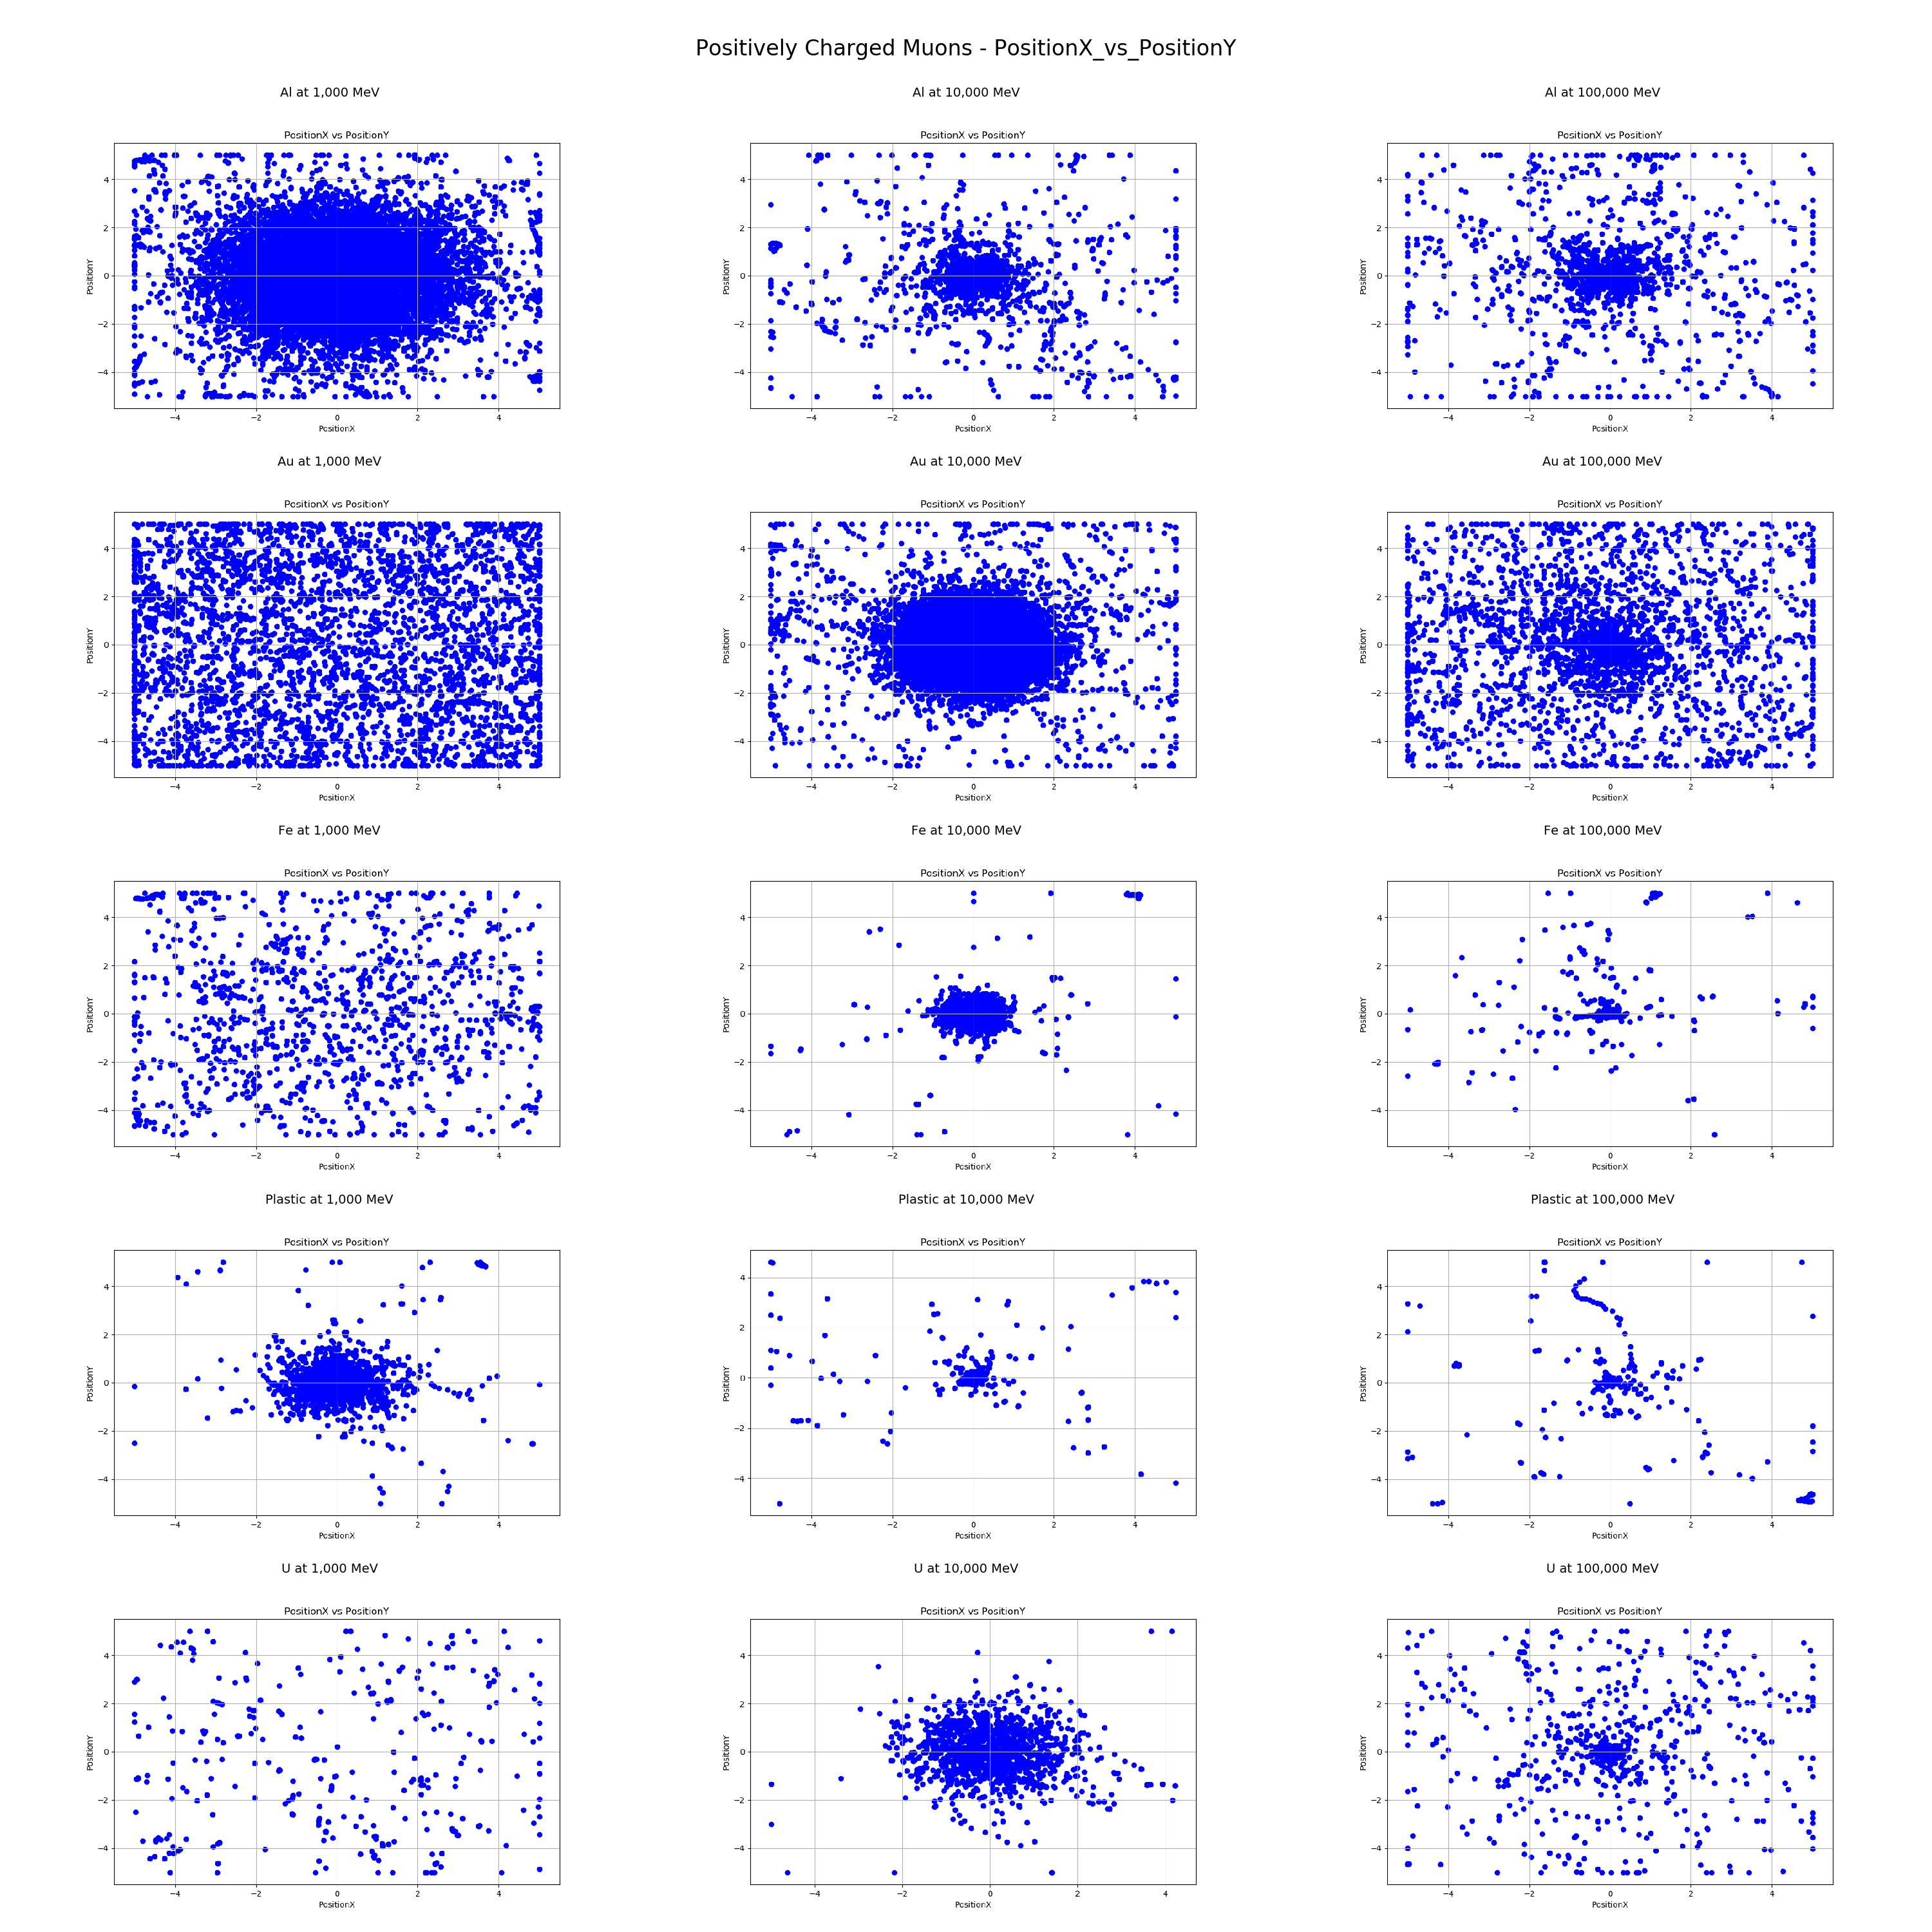
\includegraphics[width=\textwidth]{Combined Plots/PositionX_vs_PositionY_mu+.png}
                \footnotesize{Starts off as scattered everywhere and then concentrates into one point.}
        \end{figure}
    \end{minipage}
\end{itemize}
\end{frame}

%------------------------------------------------

\begin{frame}
\frametitle{Negatively Charged Muons (mu-) - PositionX vs PositionY}
\begin{itemize}
    \item 
    \begin{minipage}{0.5\textwidth}
        \begin{figure}
            \centering
            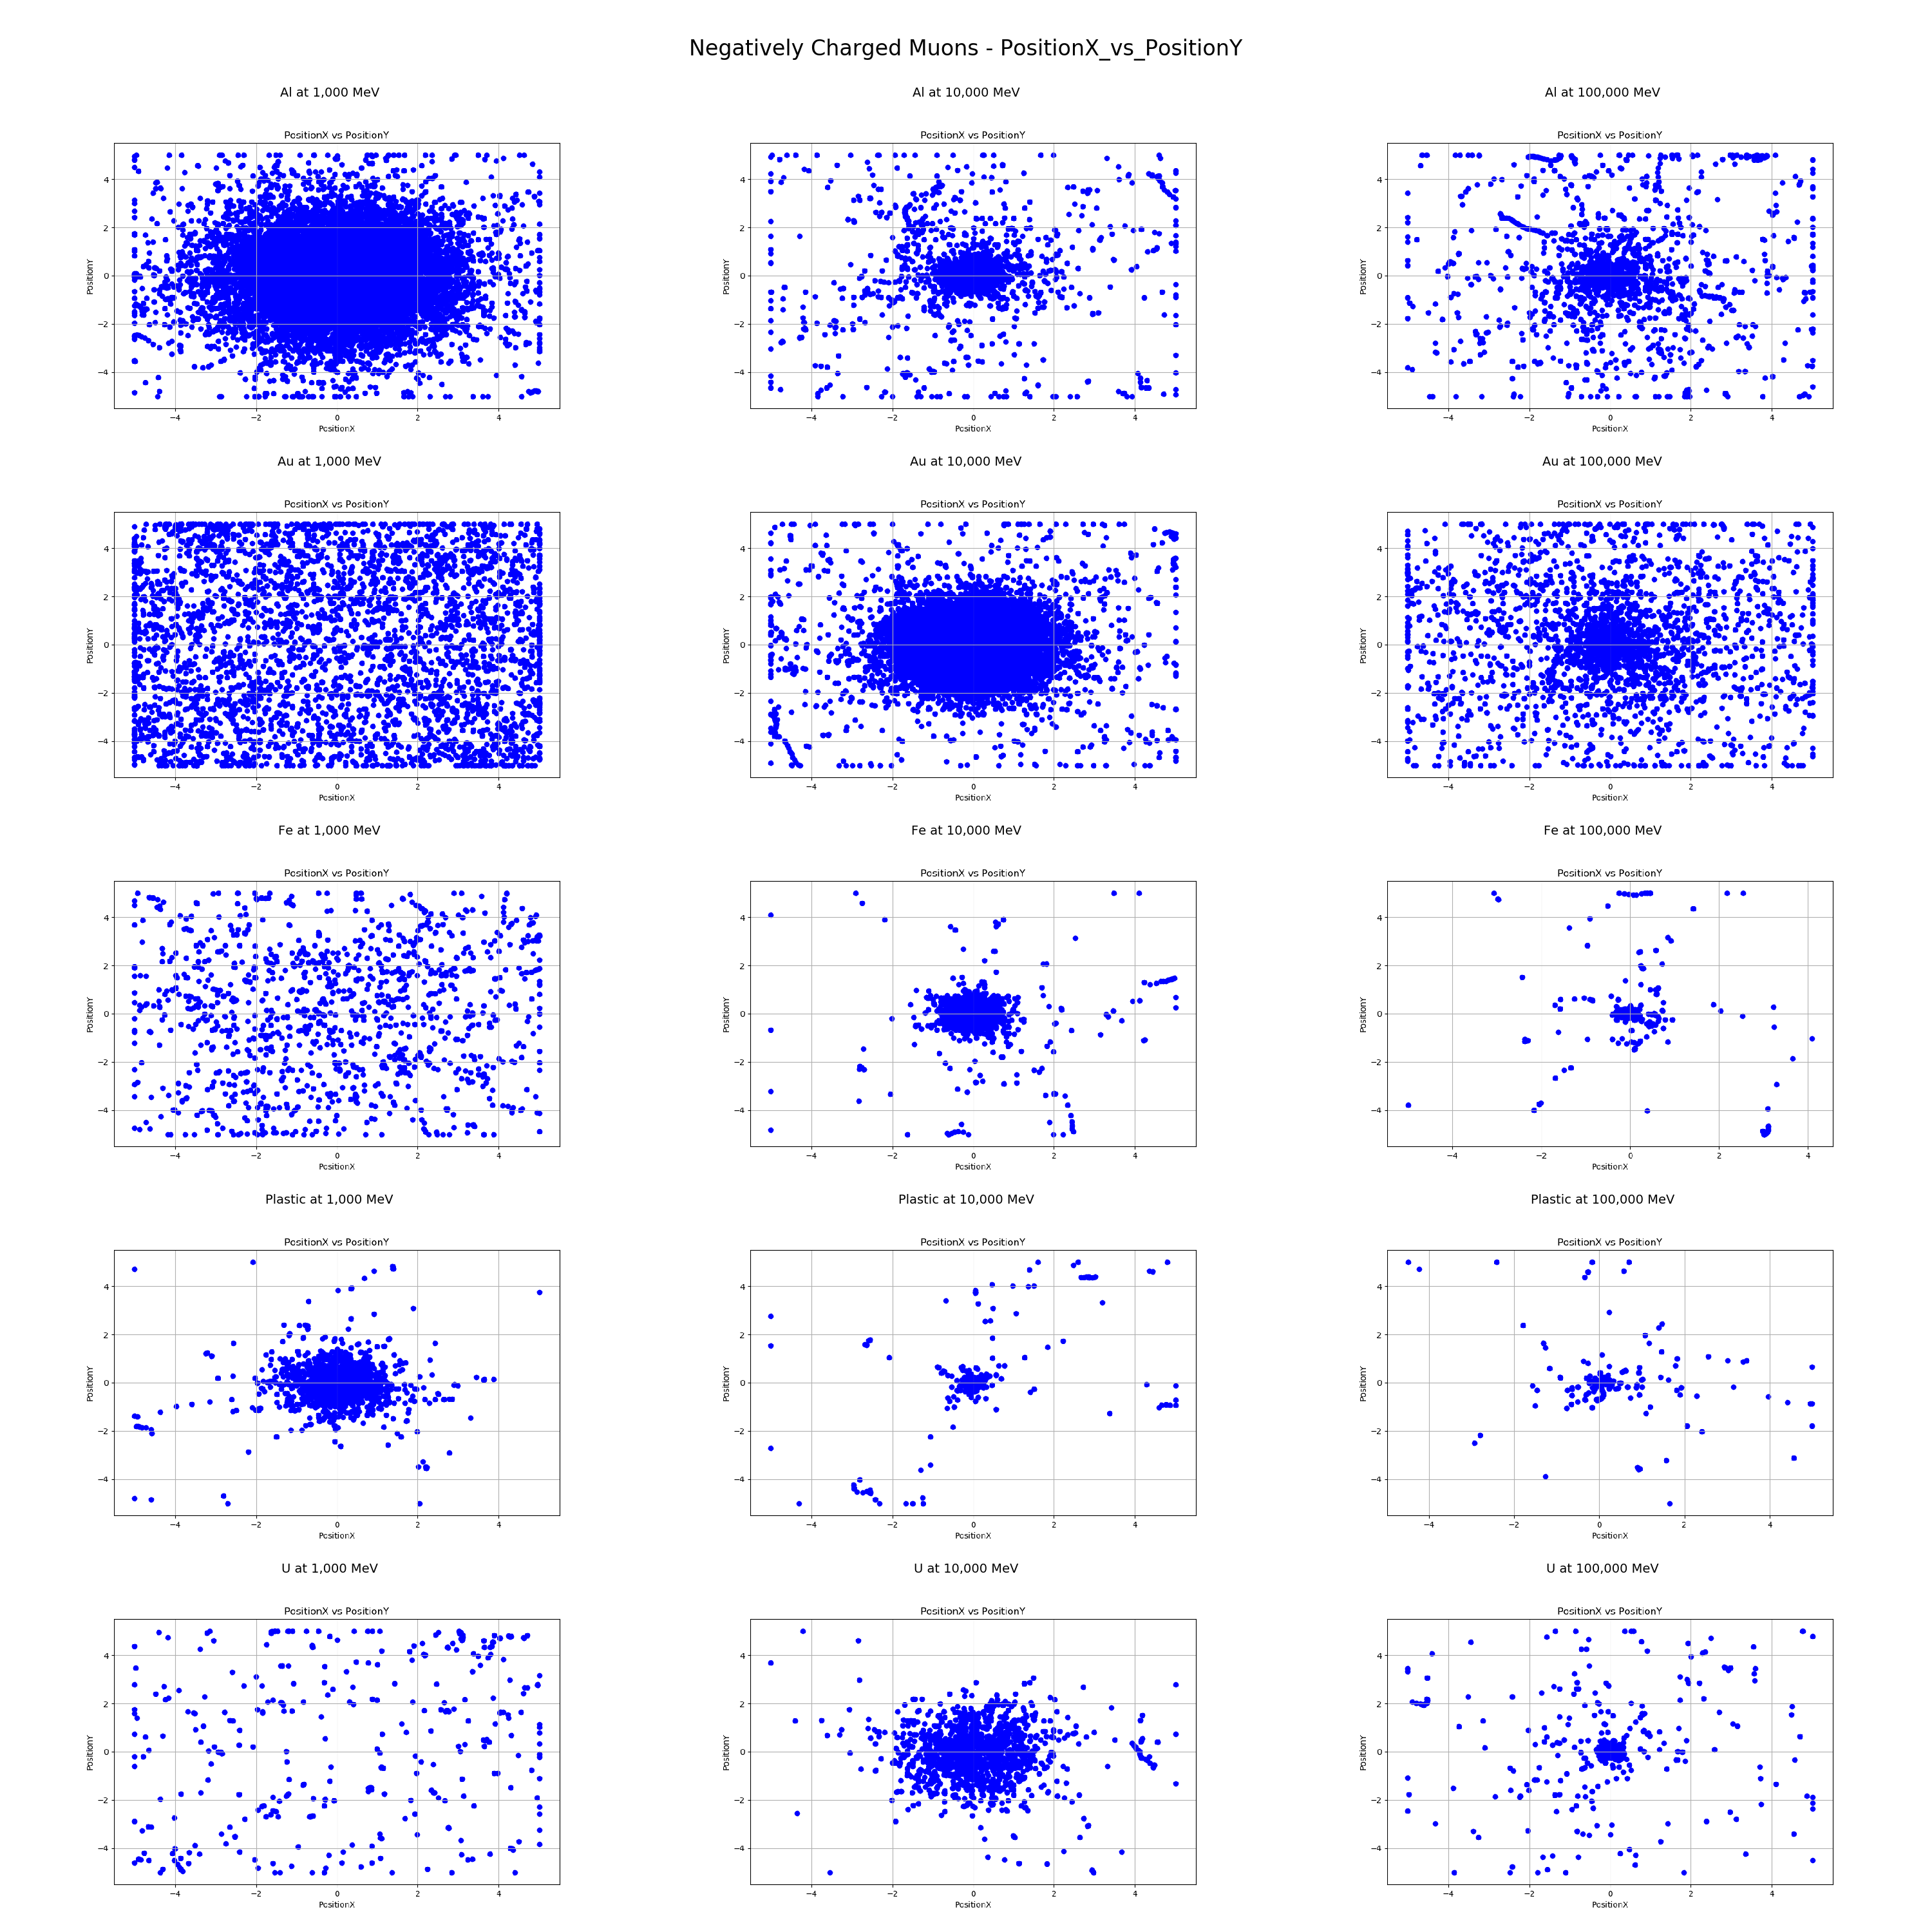
\includegraphics[width=\textwidth]{Combined Plots/PositionX_vs_PositionY_mu-.png}
            \footnotesize{Starts off as scattered everywhere and then concentrates into one point.}
        \end{figure}
    \end{minipage}
\end{itemize}
\end{frame}

%------------------------------------------------

\begin{frame}
\frametitle{Proton (p) - Momentum vs f(Momentum)}
\begin{itemize}
    \item 
    \begin{minipage}{0.5\textwidth}
        \begin{figure}
            \centering
            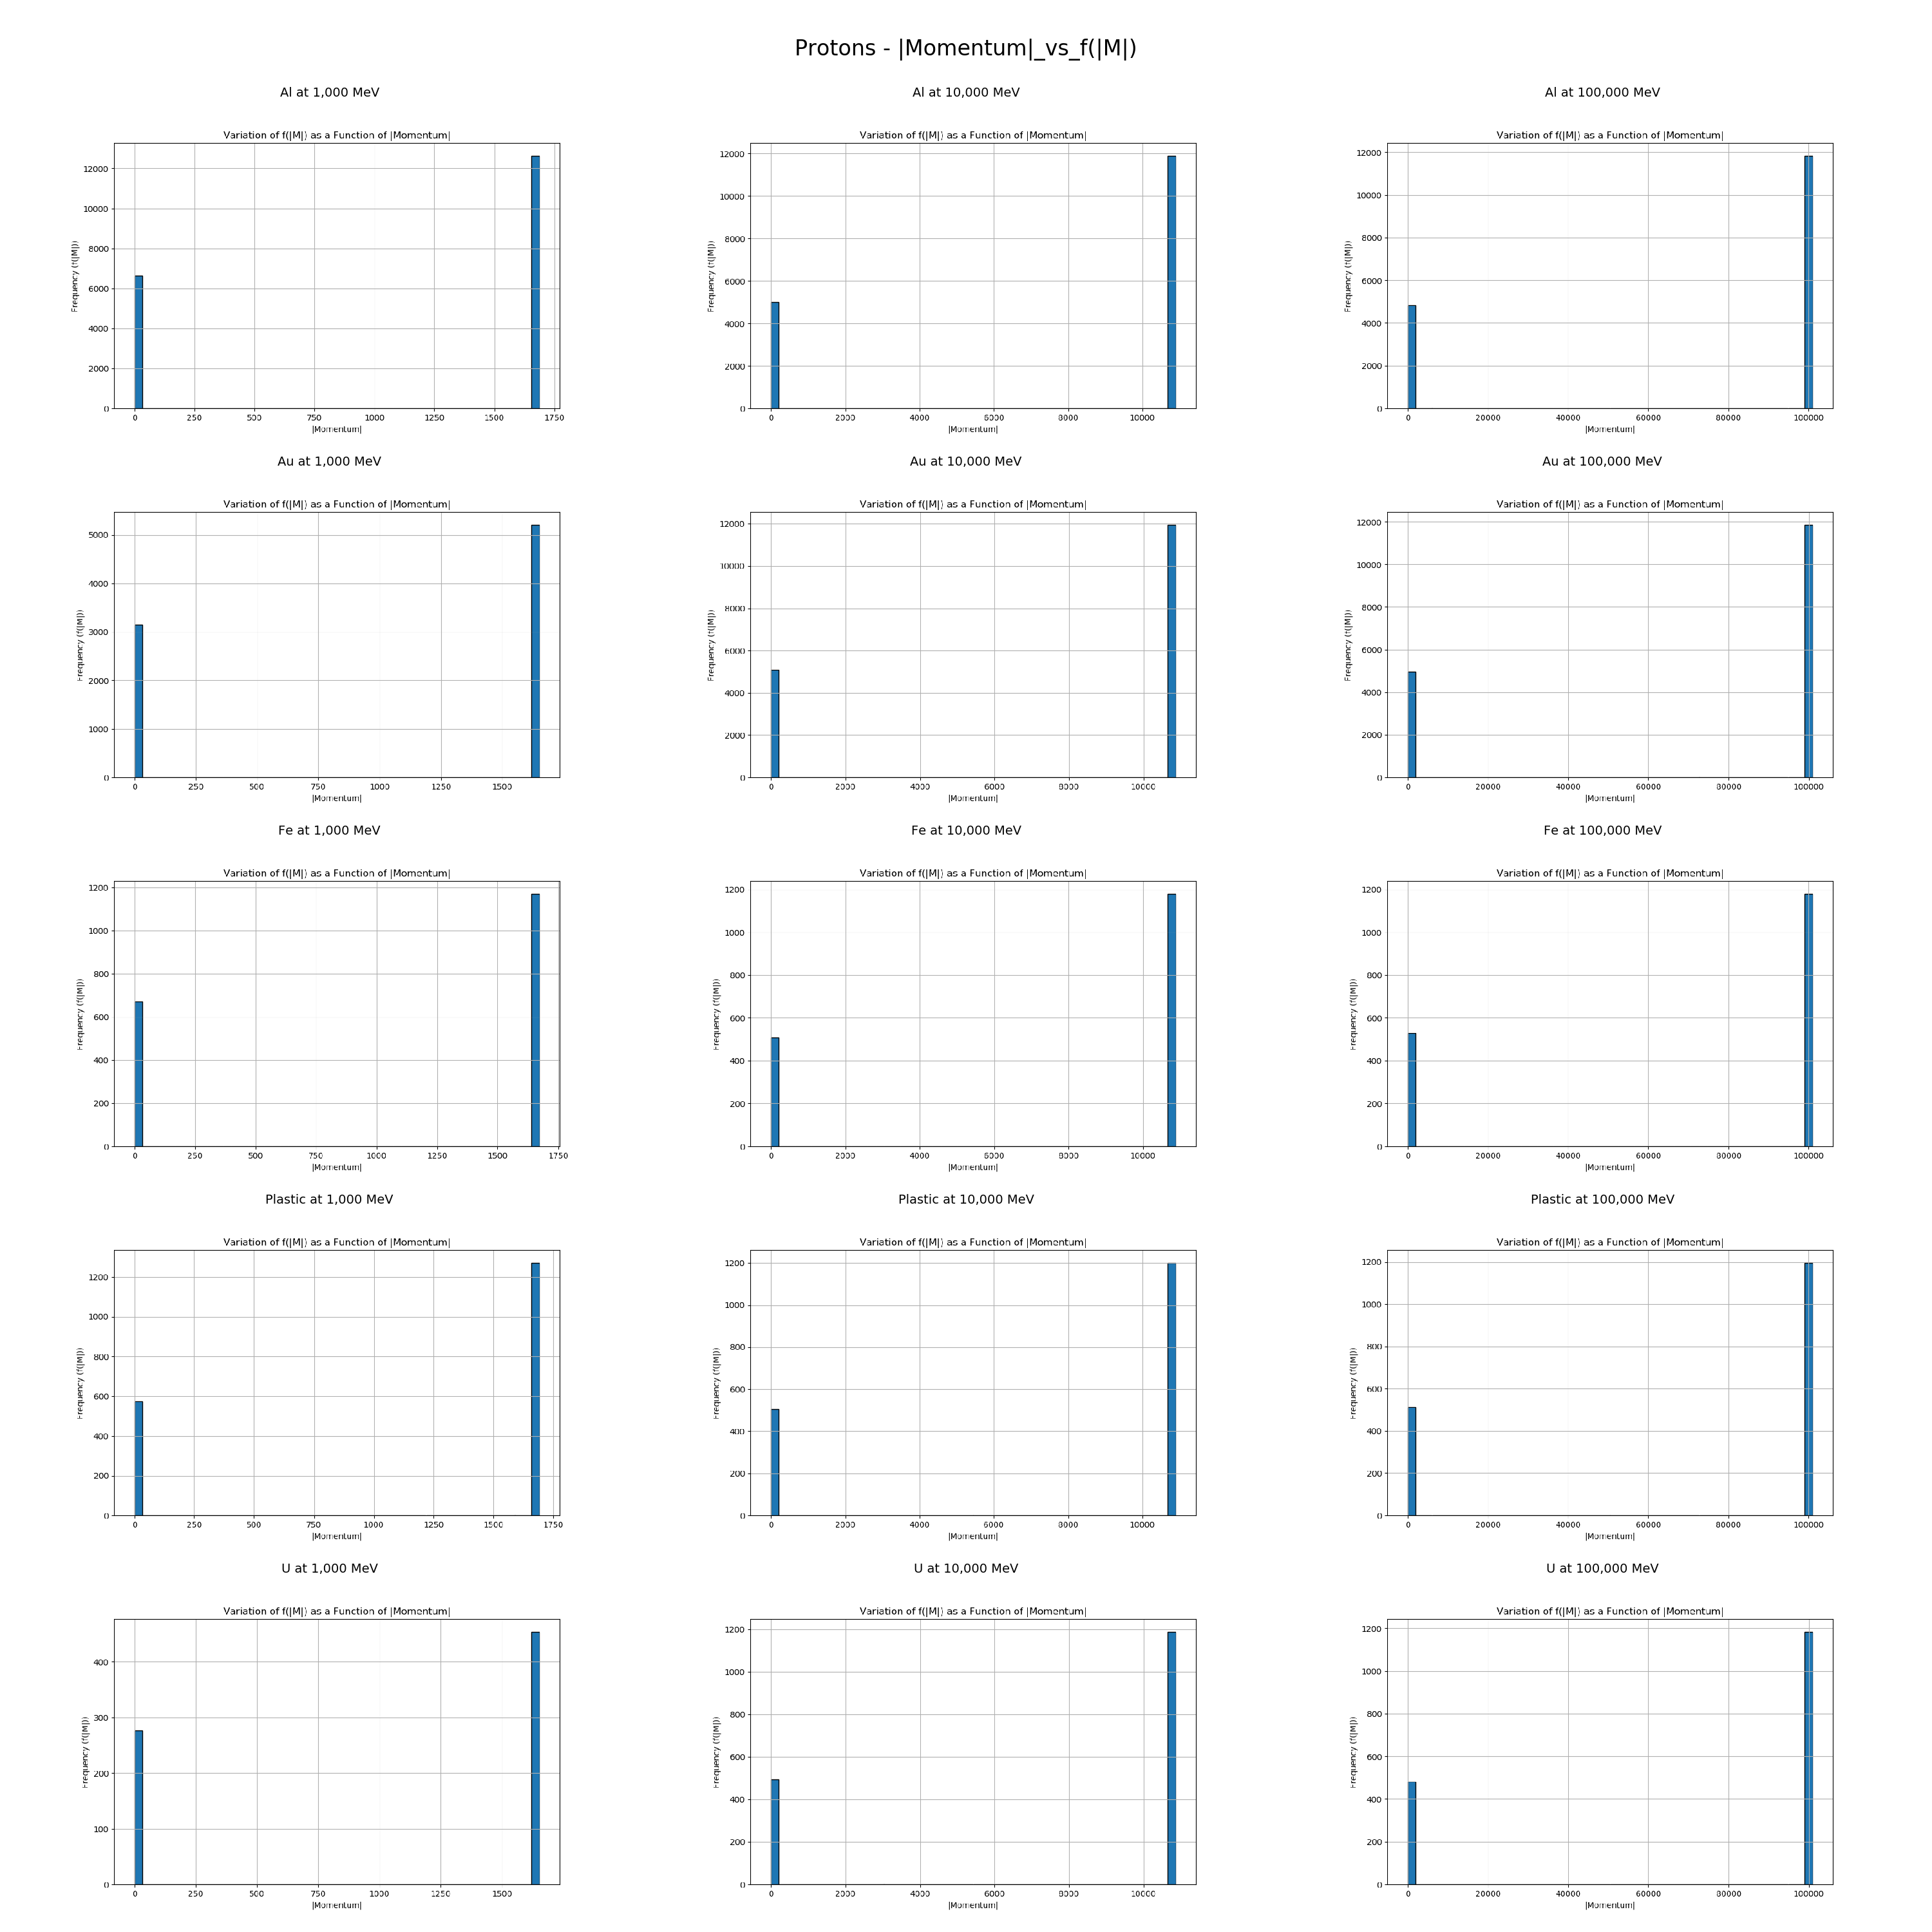
\includegraphics[width=\textwidth]{Combined Plots/|Momentum|_vs_f(|M|)_p.png}
            \footnotesize{Momentum is usually very frequent between 1500-1750 MeV/c.}
        \end{figure}
    \end{minipage}
\end{itemize}
\end{frame}

%------------------------------------------------

\begin{frame}
\frametitle{Electron (e-) - Momentum vs f(Momentum)}
\begin{itemize}
    \item 
    \begin{minipage}{0.5\textwidth}
        \begin{figure}
            \centering
            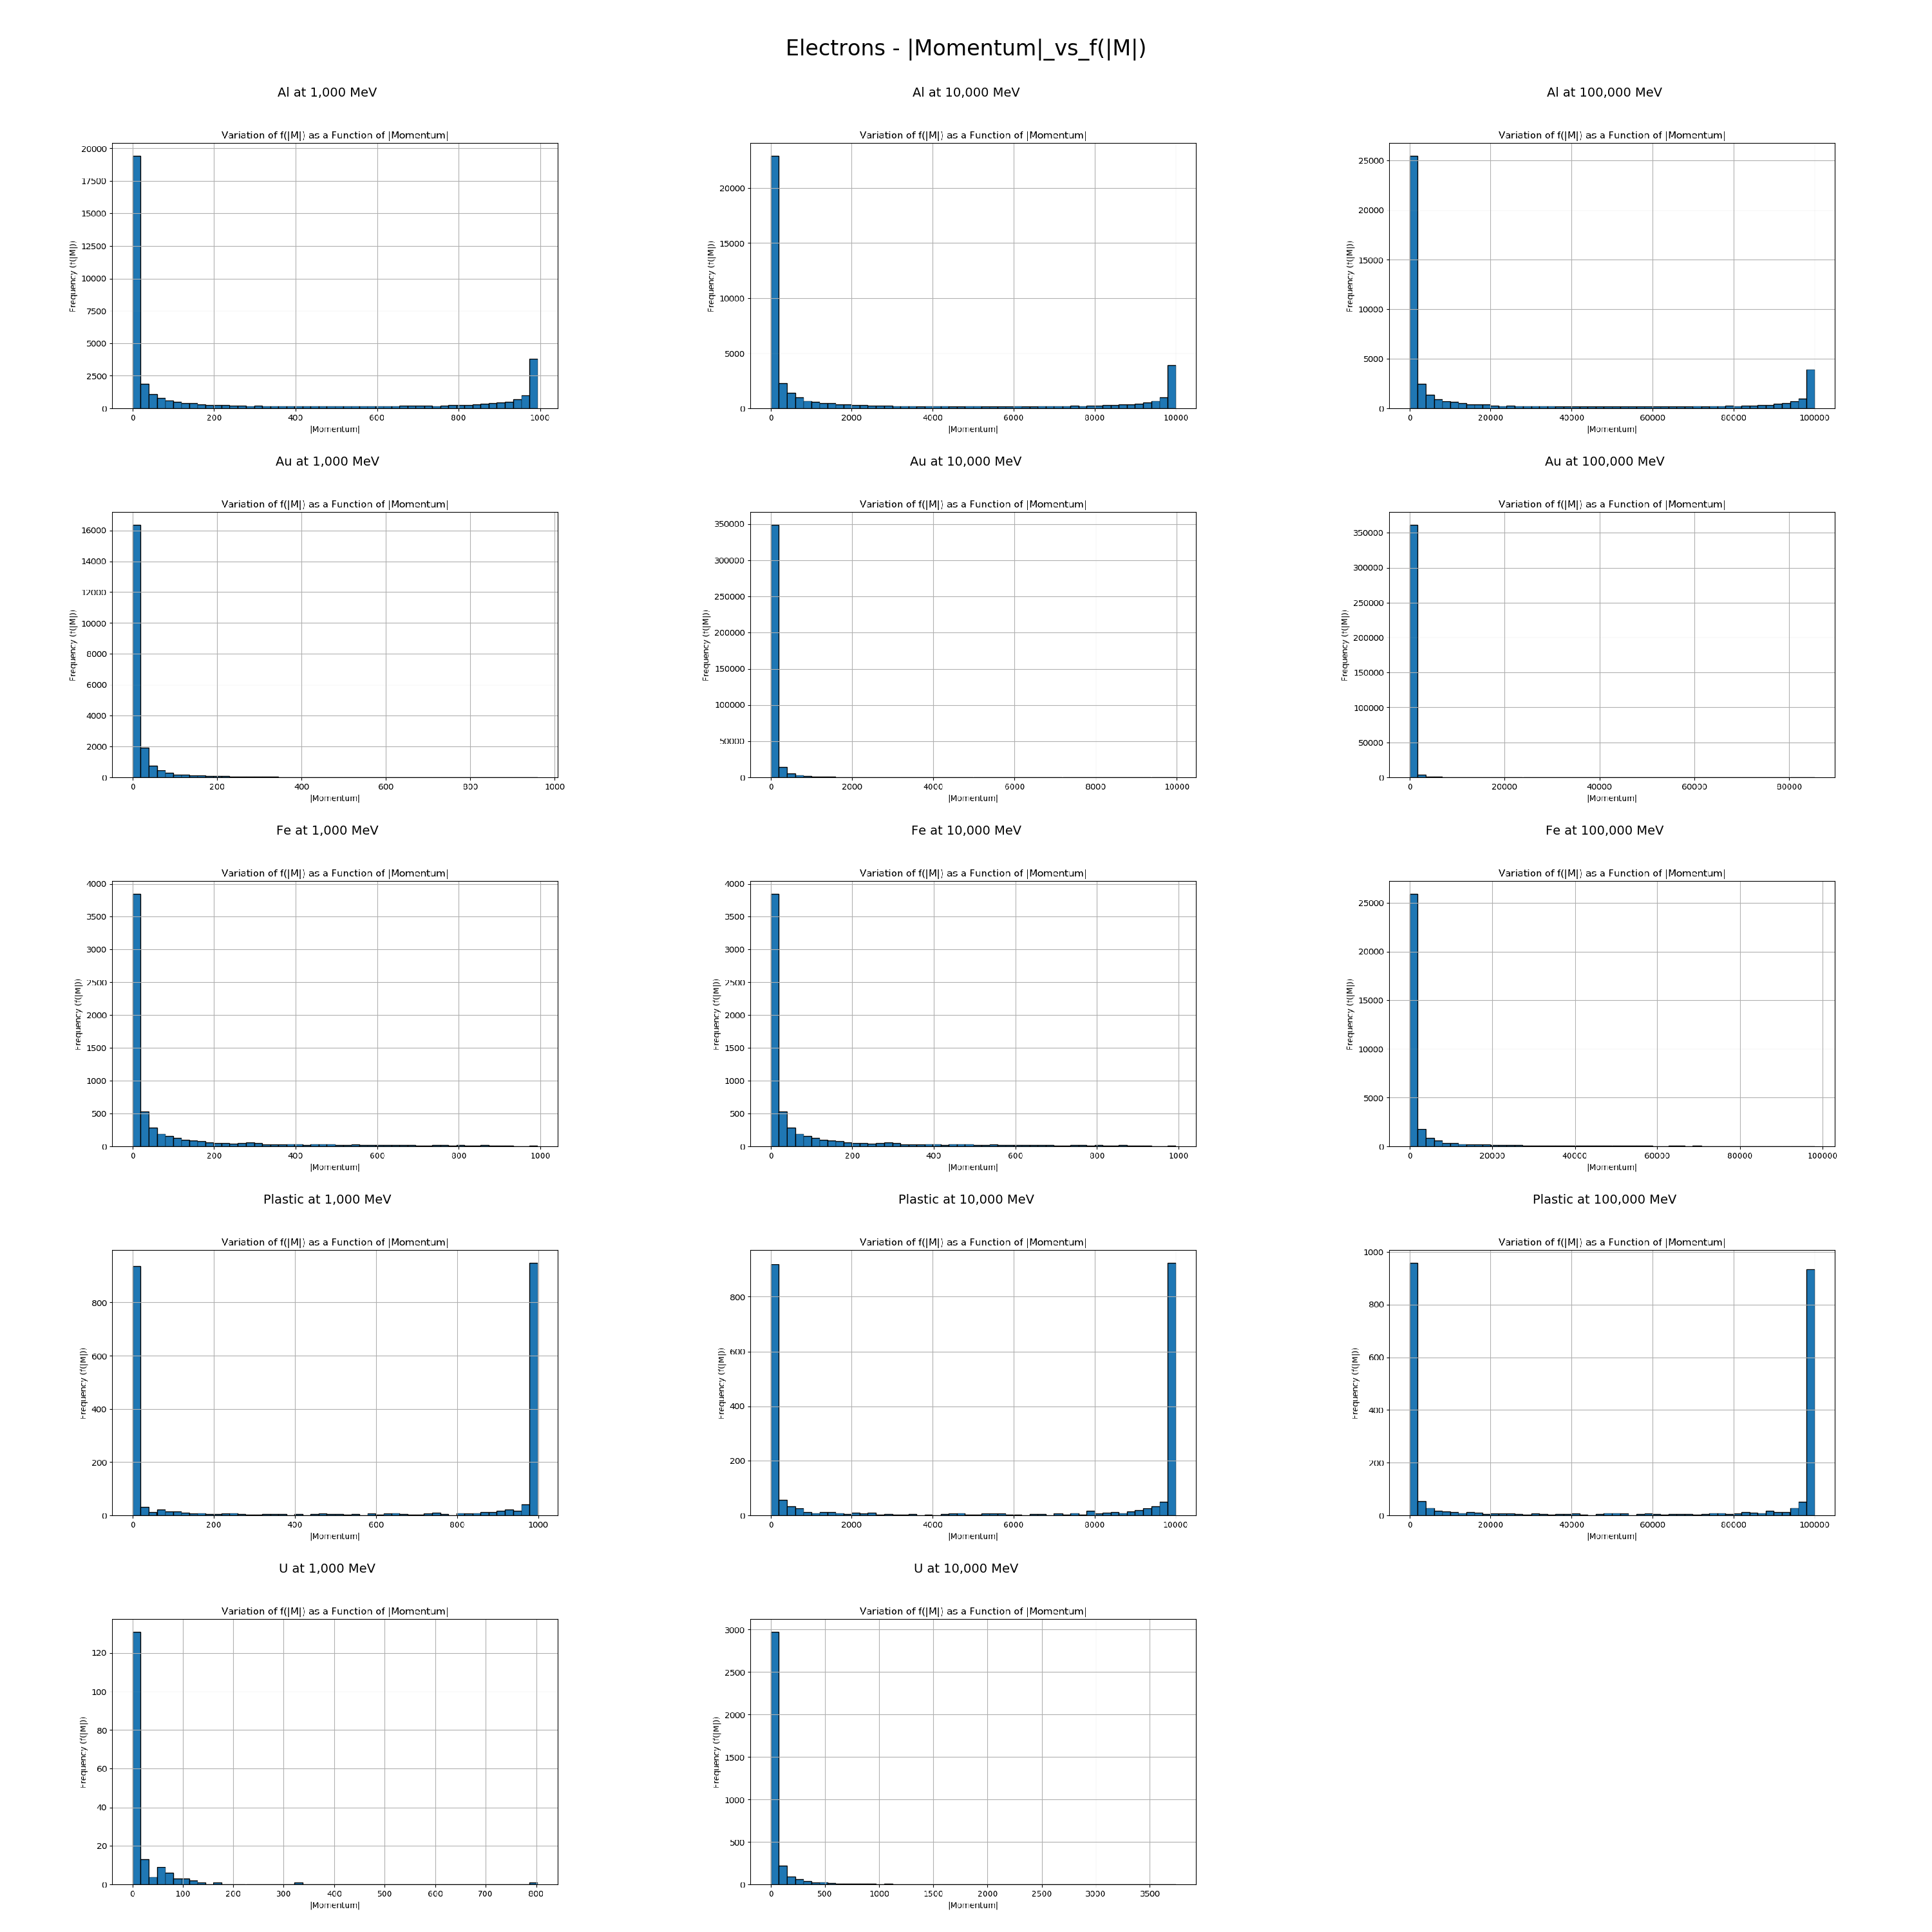
\includegraphics[width=\textwidth]{Combined Plots/|Momentum|_vs_f(|M|)_e-.png}
            \footnotesize{Momentum depends on which material you are looking at.}
        \end{figure}
    \end{minipage}
\end{itemize}
\end{frame}

%------------------------------------------------

\begin{frame}
\frametitle{Positively Charged Muons (mu+) - Momentum vs f(Momentum)}
\begin{itemize}
    \item 
    \begin{minipage}{0.5\textwidth}
        \begin{figure}
            \centering
            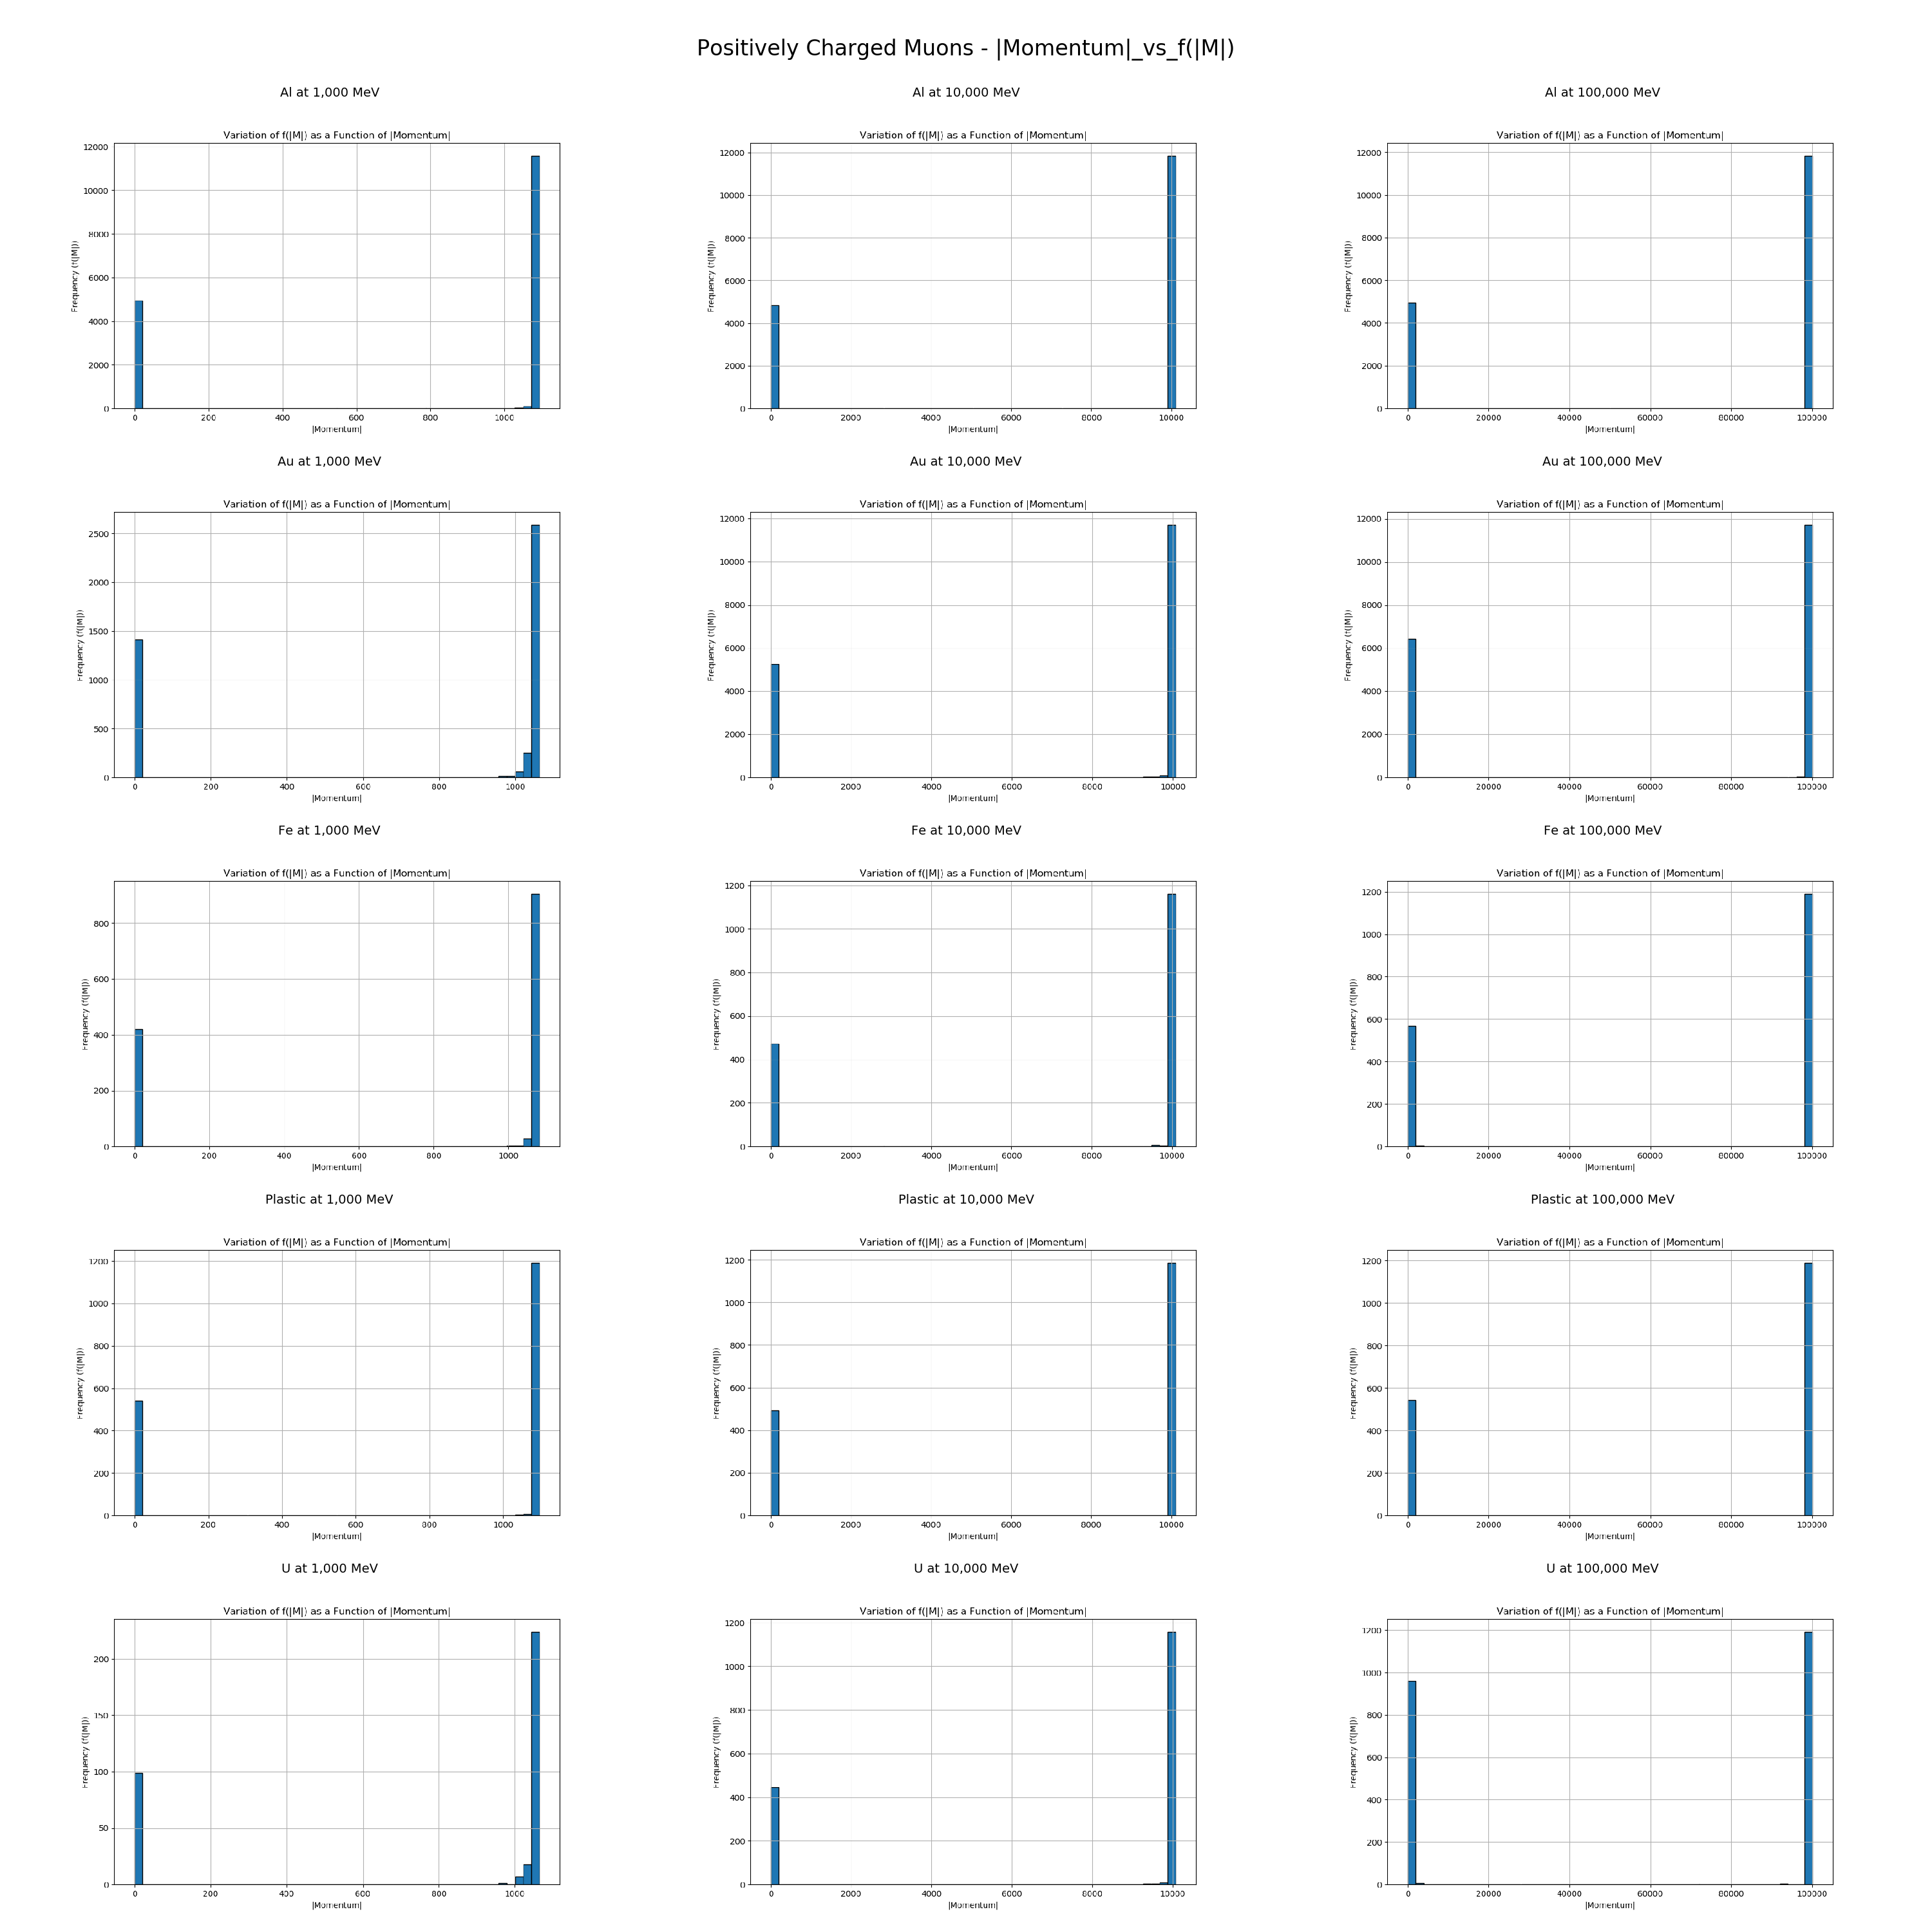
\includegraphics[width=\textwidth]{Combined Plots/|Momentum|_vs_f(|M|)_mu+.png}
            \footnotesize{Momentum is usually very frequent between 1500-1750 MeV/c for 10,000 MeV and 100,000 MeV. It depends what material it is for 1,000 MeV.}
        \end{figure}
    \end{minipage}
\end{itemize}
\end{frame}

%------------------------------------------------

\begin{frame}
\frametitle{Negatively Charged Electrons (mu-) - Momentum vs f(Momentum)}
\begin{itemize}
    \item 
    \begin{minipage}{0.5\textwidth}
        \begin{figure}
            \centering
            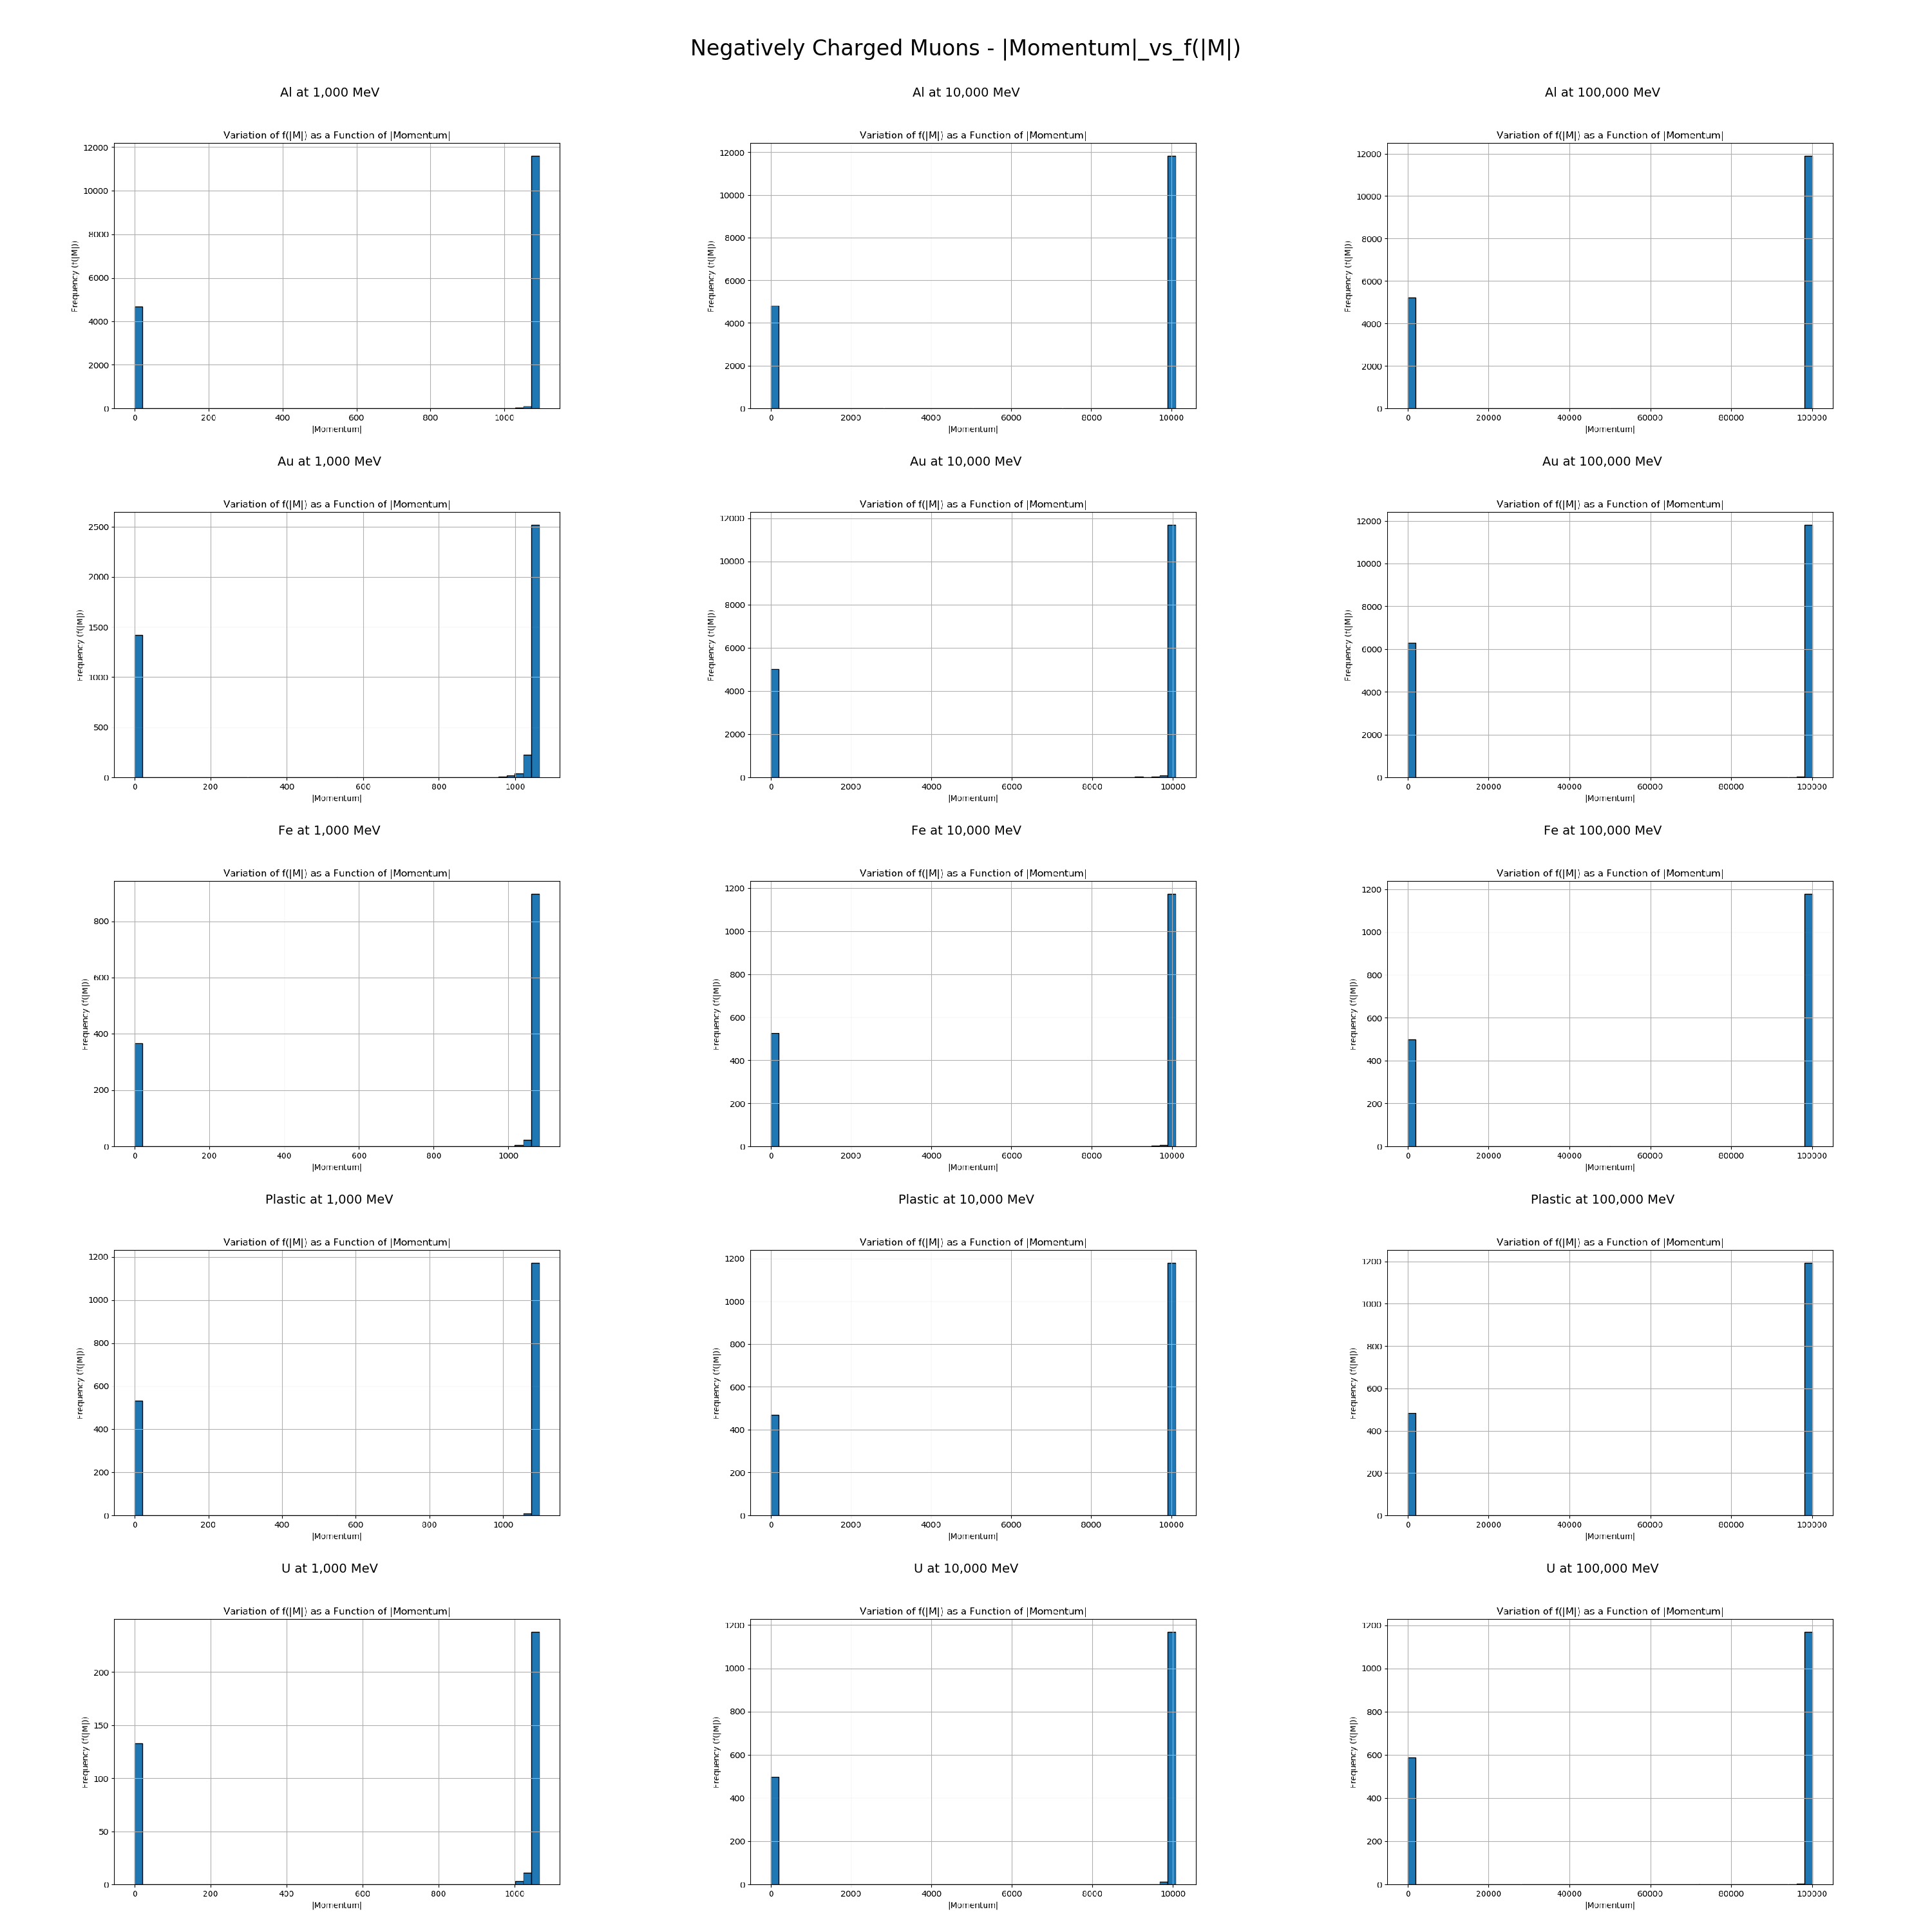
\includegraphics[width=\textwidth]{Combined Plots/|Momentum|_vs_f(|M|)_mu-.png}
            \footnotesize{Same as positively charged muons.}
        \end{figure}
    \end{minipage}
\end{itemize}
\end{frame}

%------------------------------------------------

\begin{frame}
\frametitle{Proton (p) - \# of Particles vs Radius of Detector Plane}
\begin{itemize}
    \item 
    \begin{minipage}{0.5\textwidth}
        \begin{figure}
            \centering
            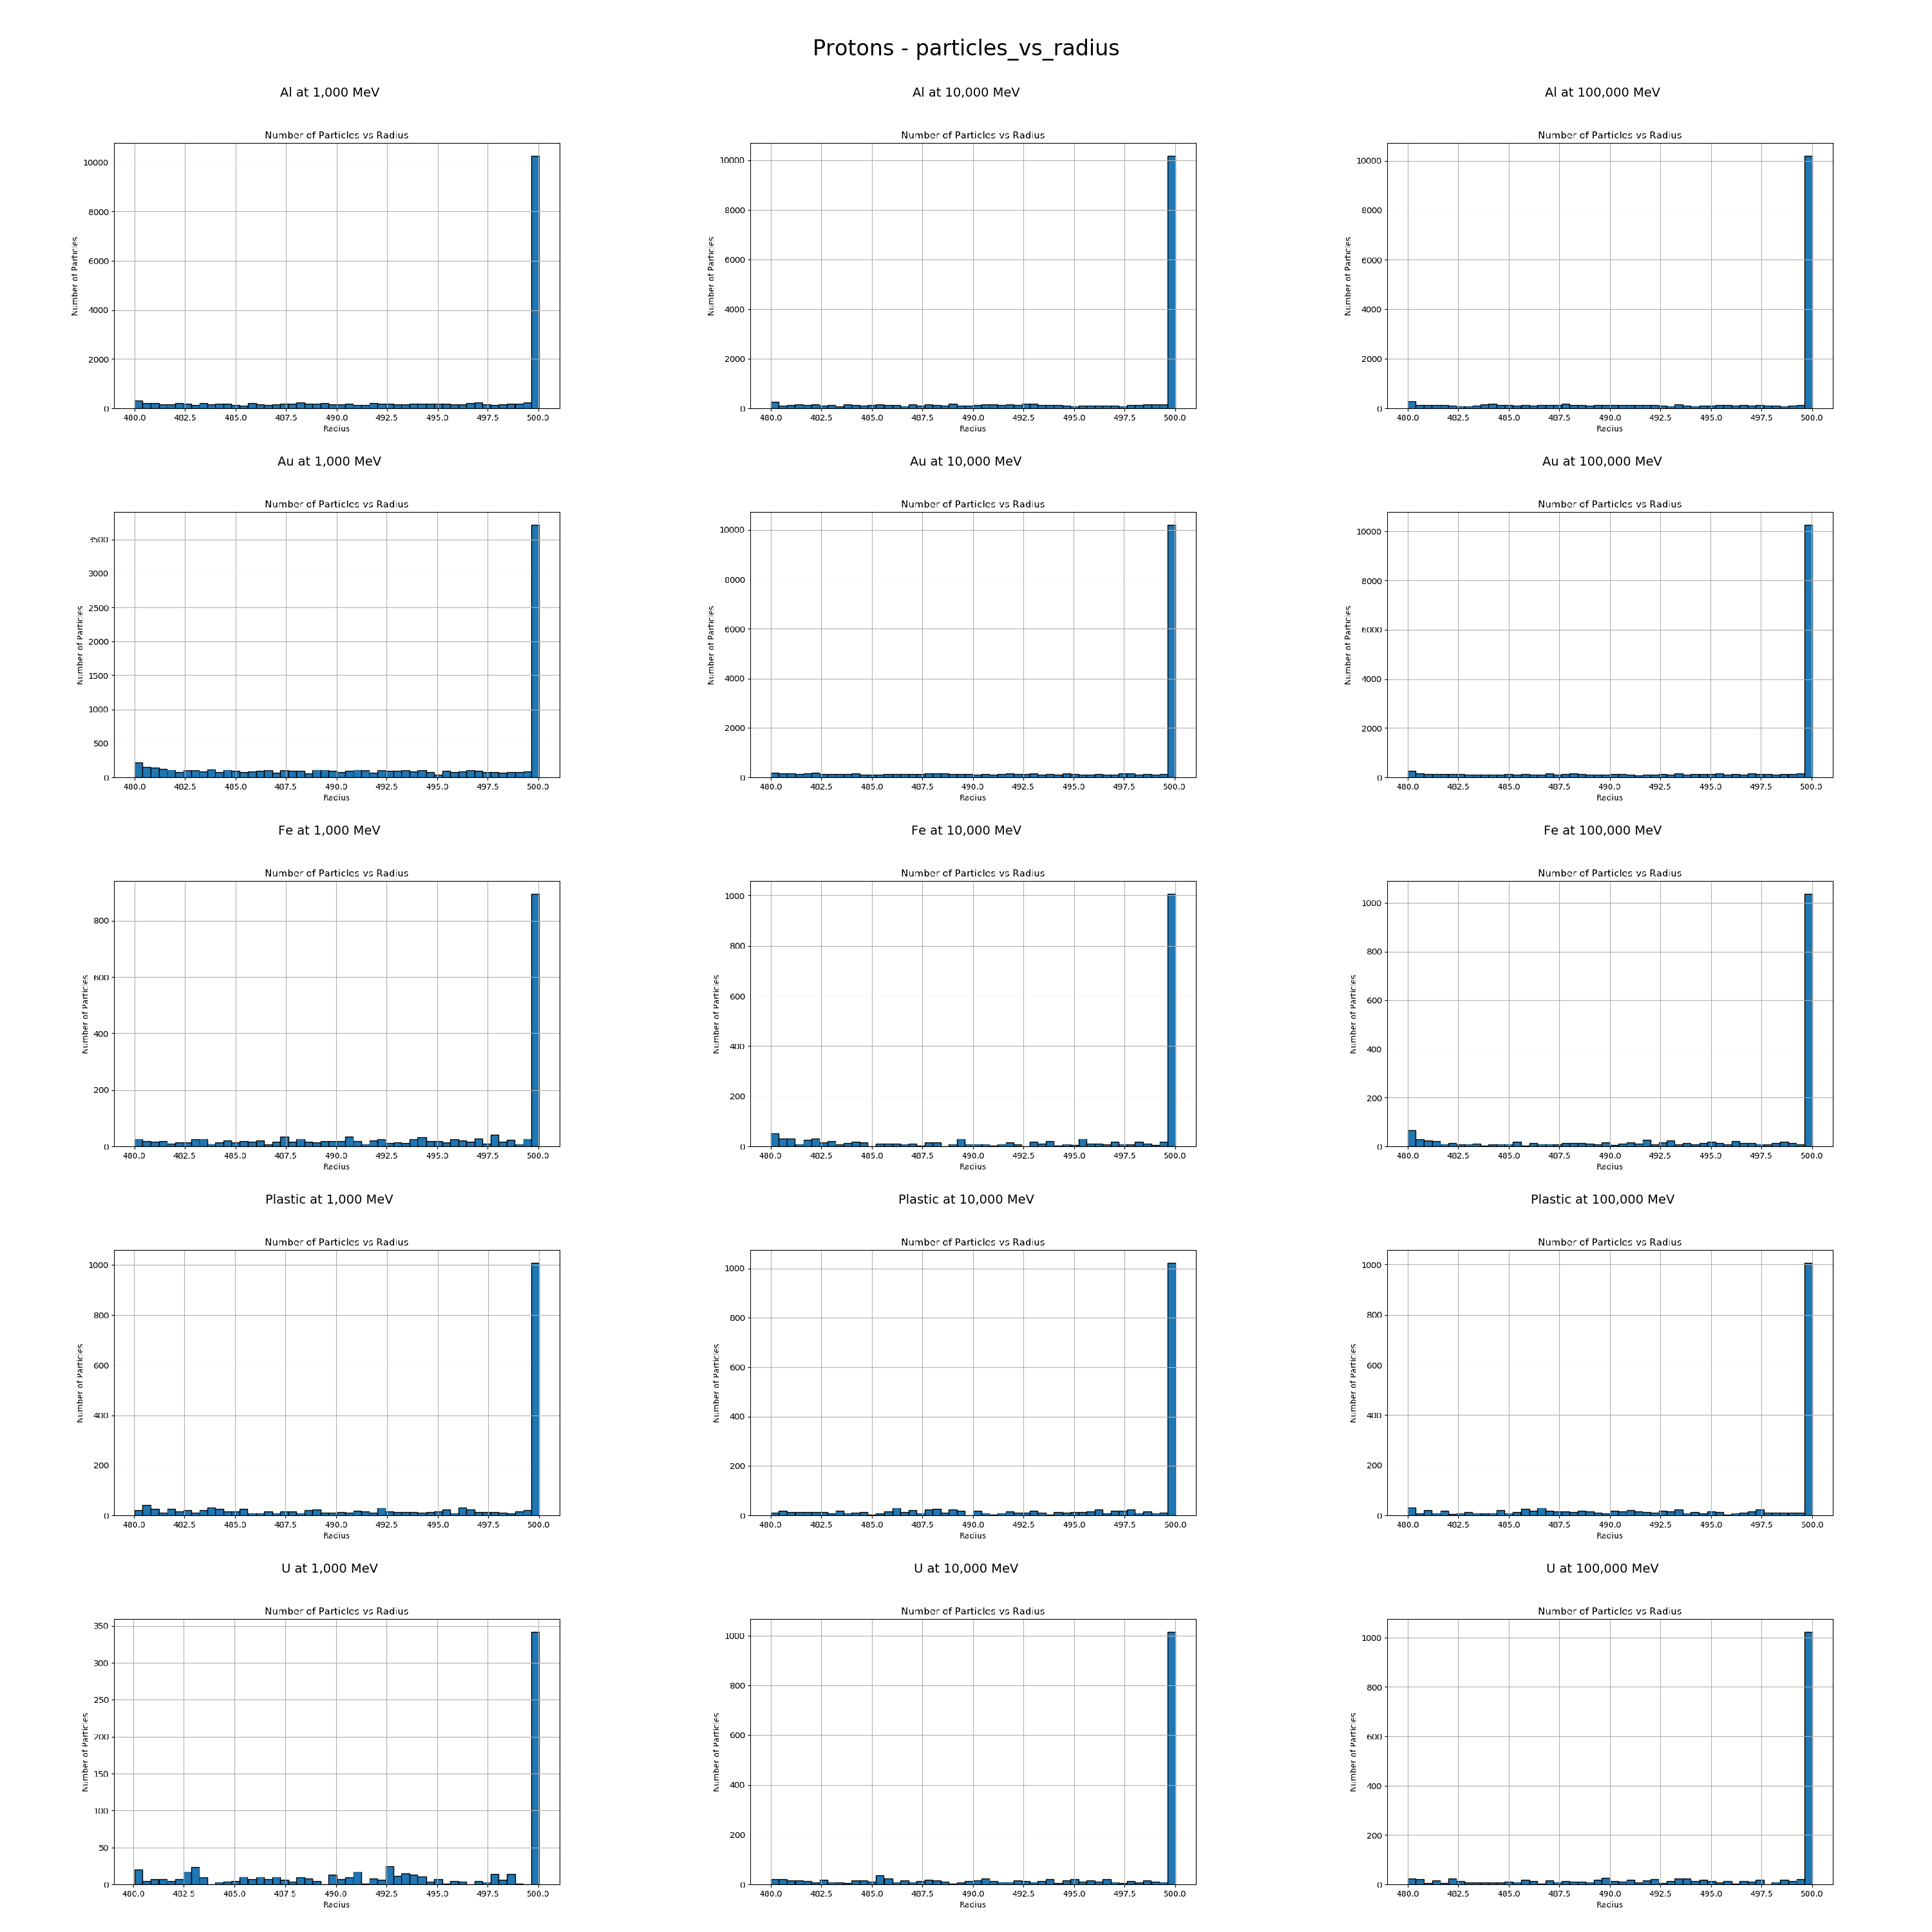
\includegraphics[width=\textwidth]{Combined Plots/particles_vs_radius_p.png}
            \footnotesize{Constant for 10,000 and 100,000 MeV, but really depends on what material you are using for 1,000 MeV.}
        \end{figure}
    \end{minipage}
\end{itemize}
\end{frame}

%------------------------------------------------

\begin{frame}
\frametitle{Electron (e-) - \# of Particles vs Radius of Detector Plane}
\begin{itemize}
    \item 
    \begin{minipage}{0.5\textwidth}
        \begin{figure}
            \centering
            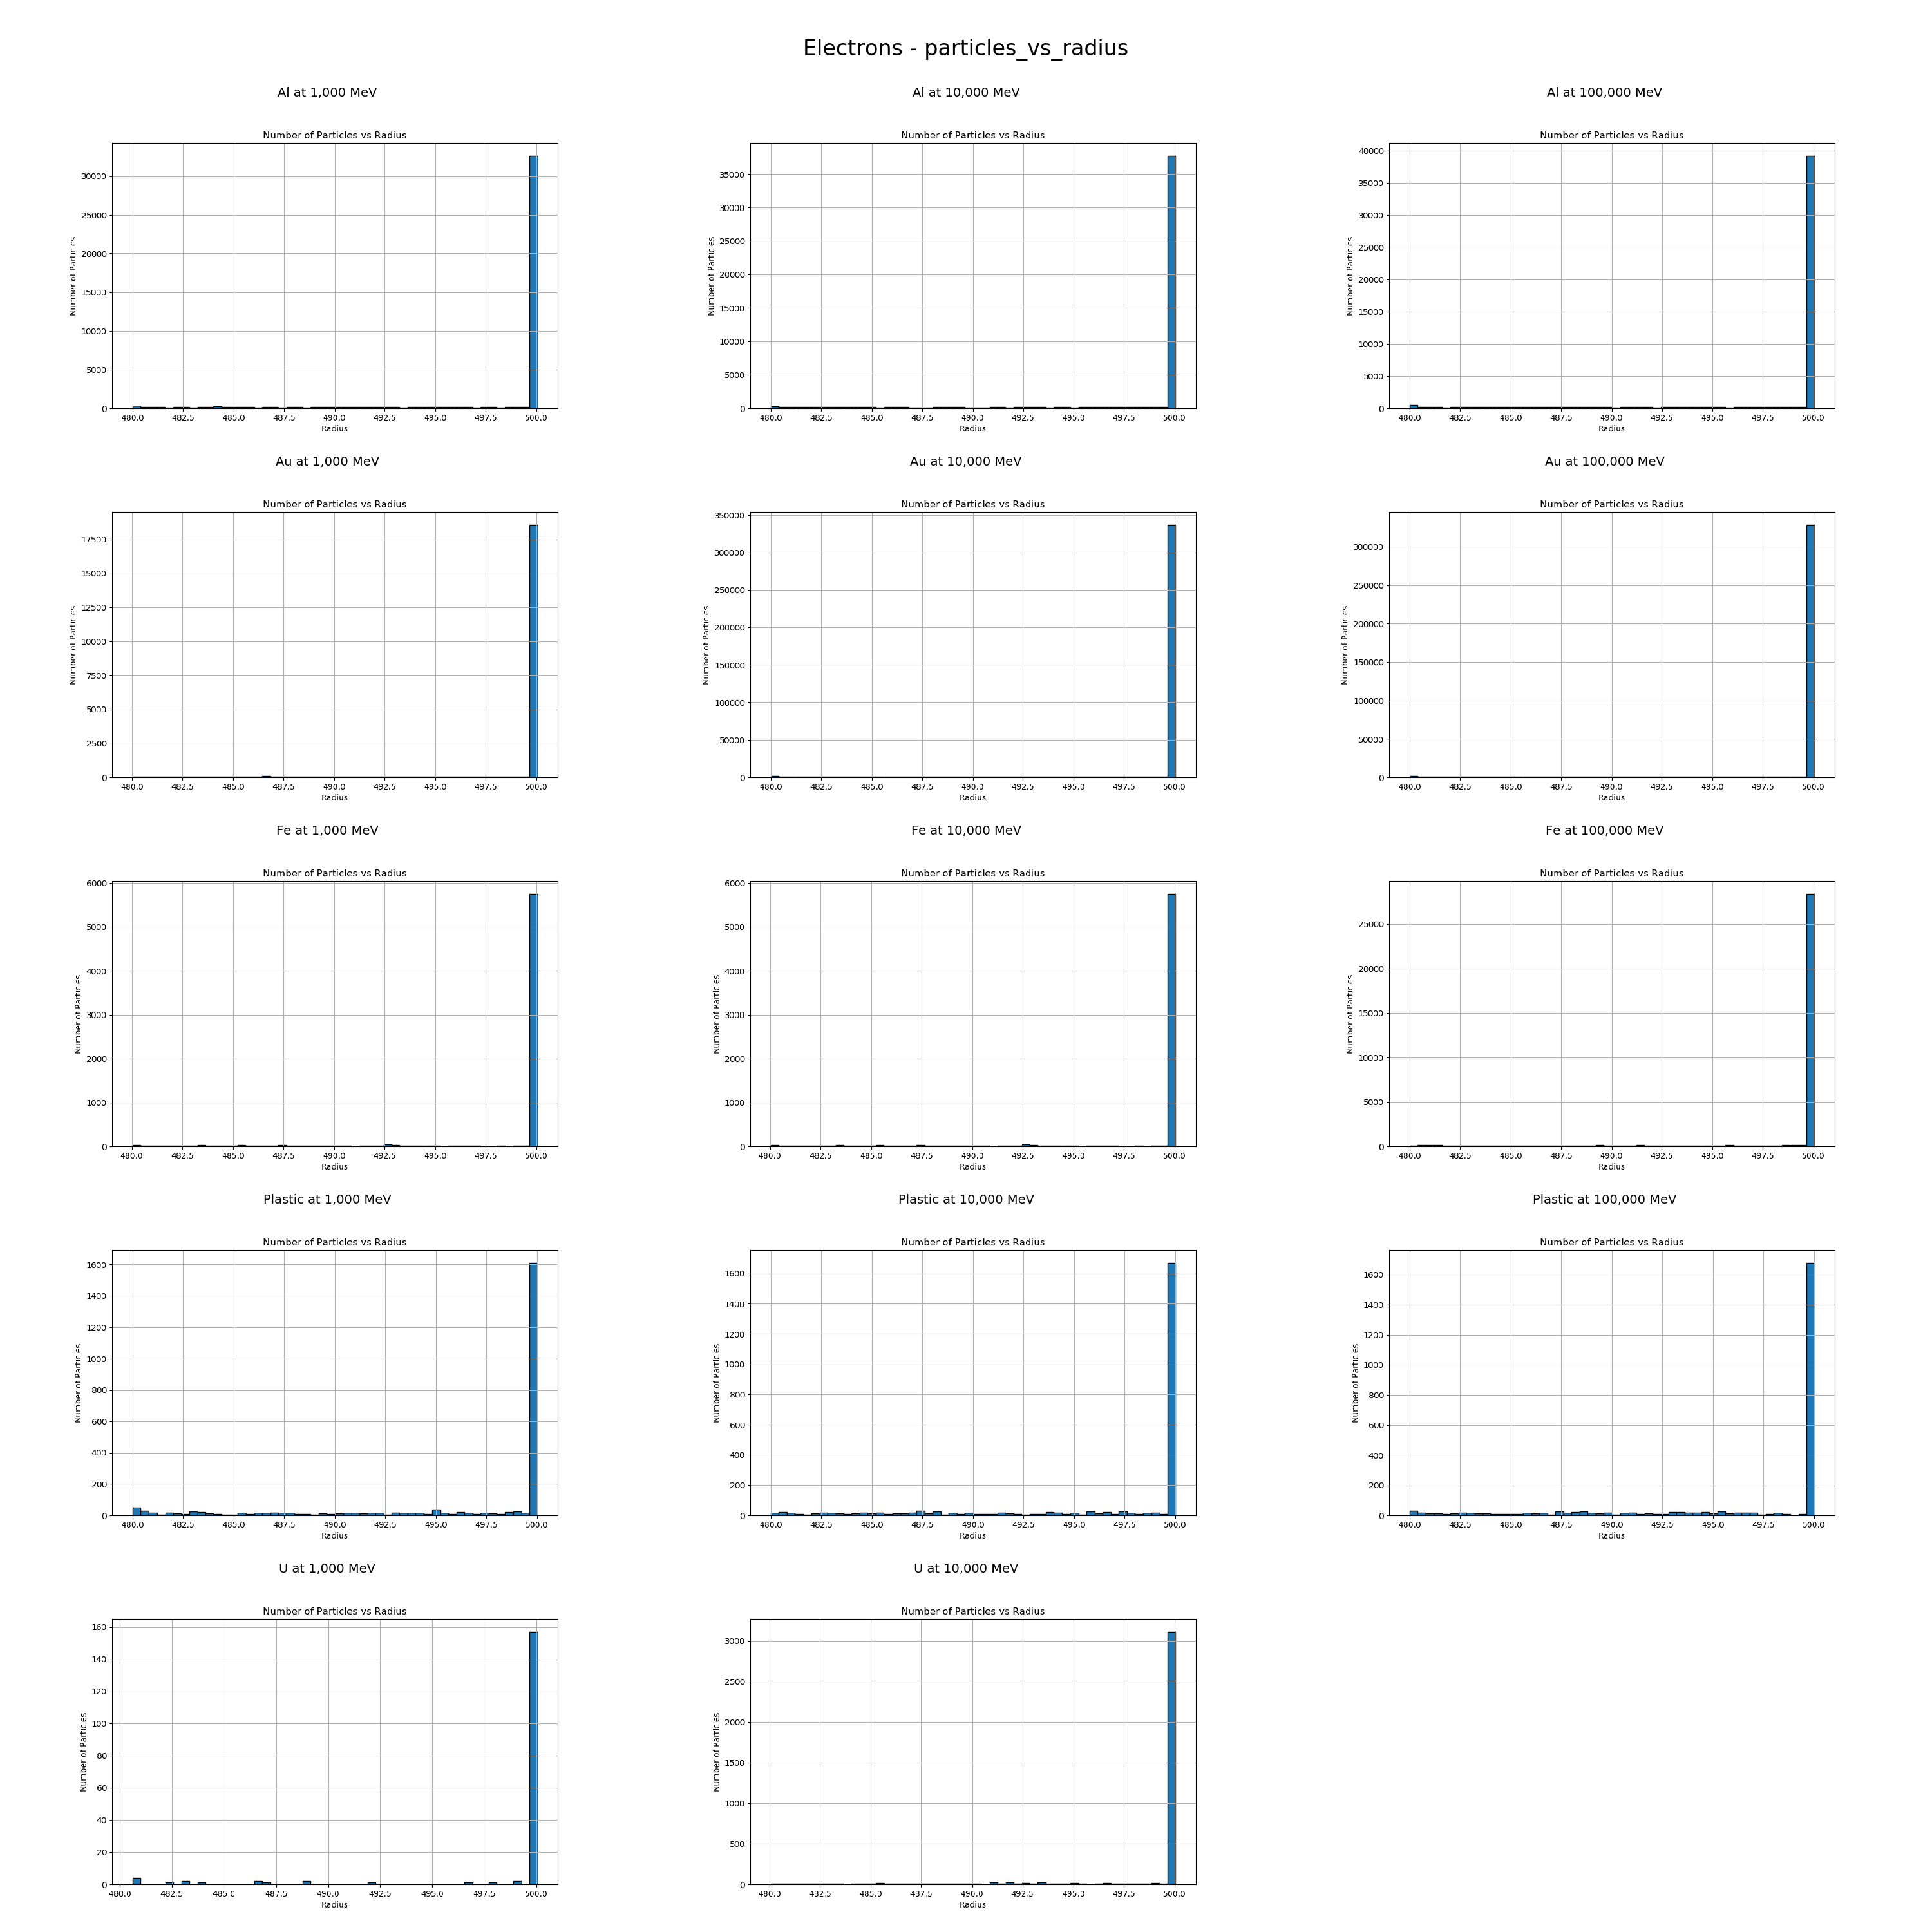
\includegraphics[width=\textwidth]{Combined Plots/particles_vs_radius_e-.png}
            \footnotesize{Very much depends on what material you are using.}
        \end{figure}
    \end{minipage}
\end{itemize}
\end{frame}

%------------------------------------------------

\begin{frame}
\frametitle{Positively Charged Muons (mu+) - \# of Particles vs Radius of Detector Plane}
\begin{itemize}
    \item 
    \begin{minipage}{0.5\textwidth}
        \begin{figure}
            \centering
            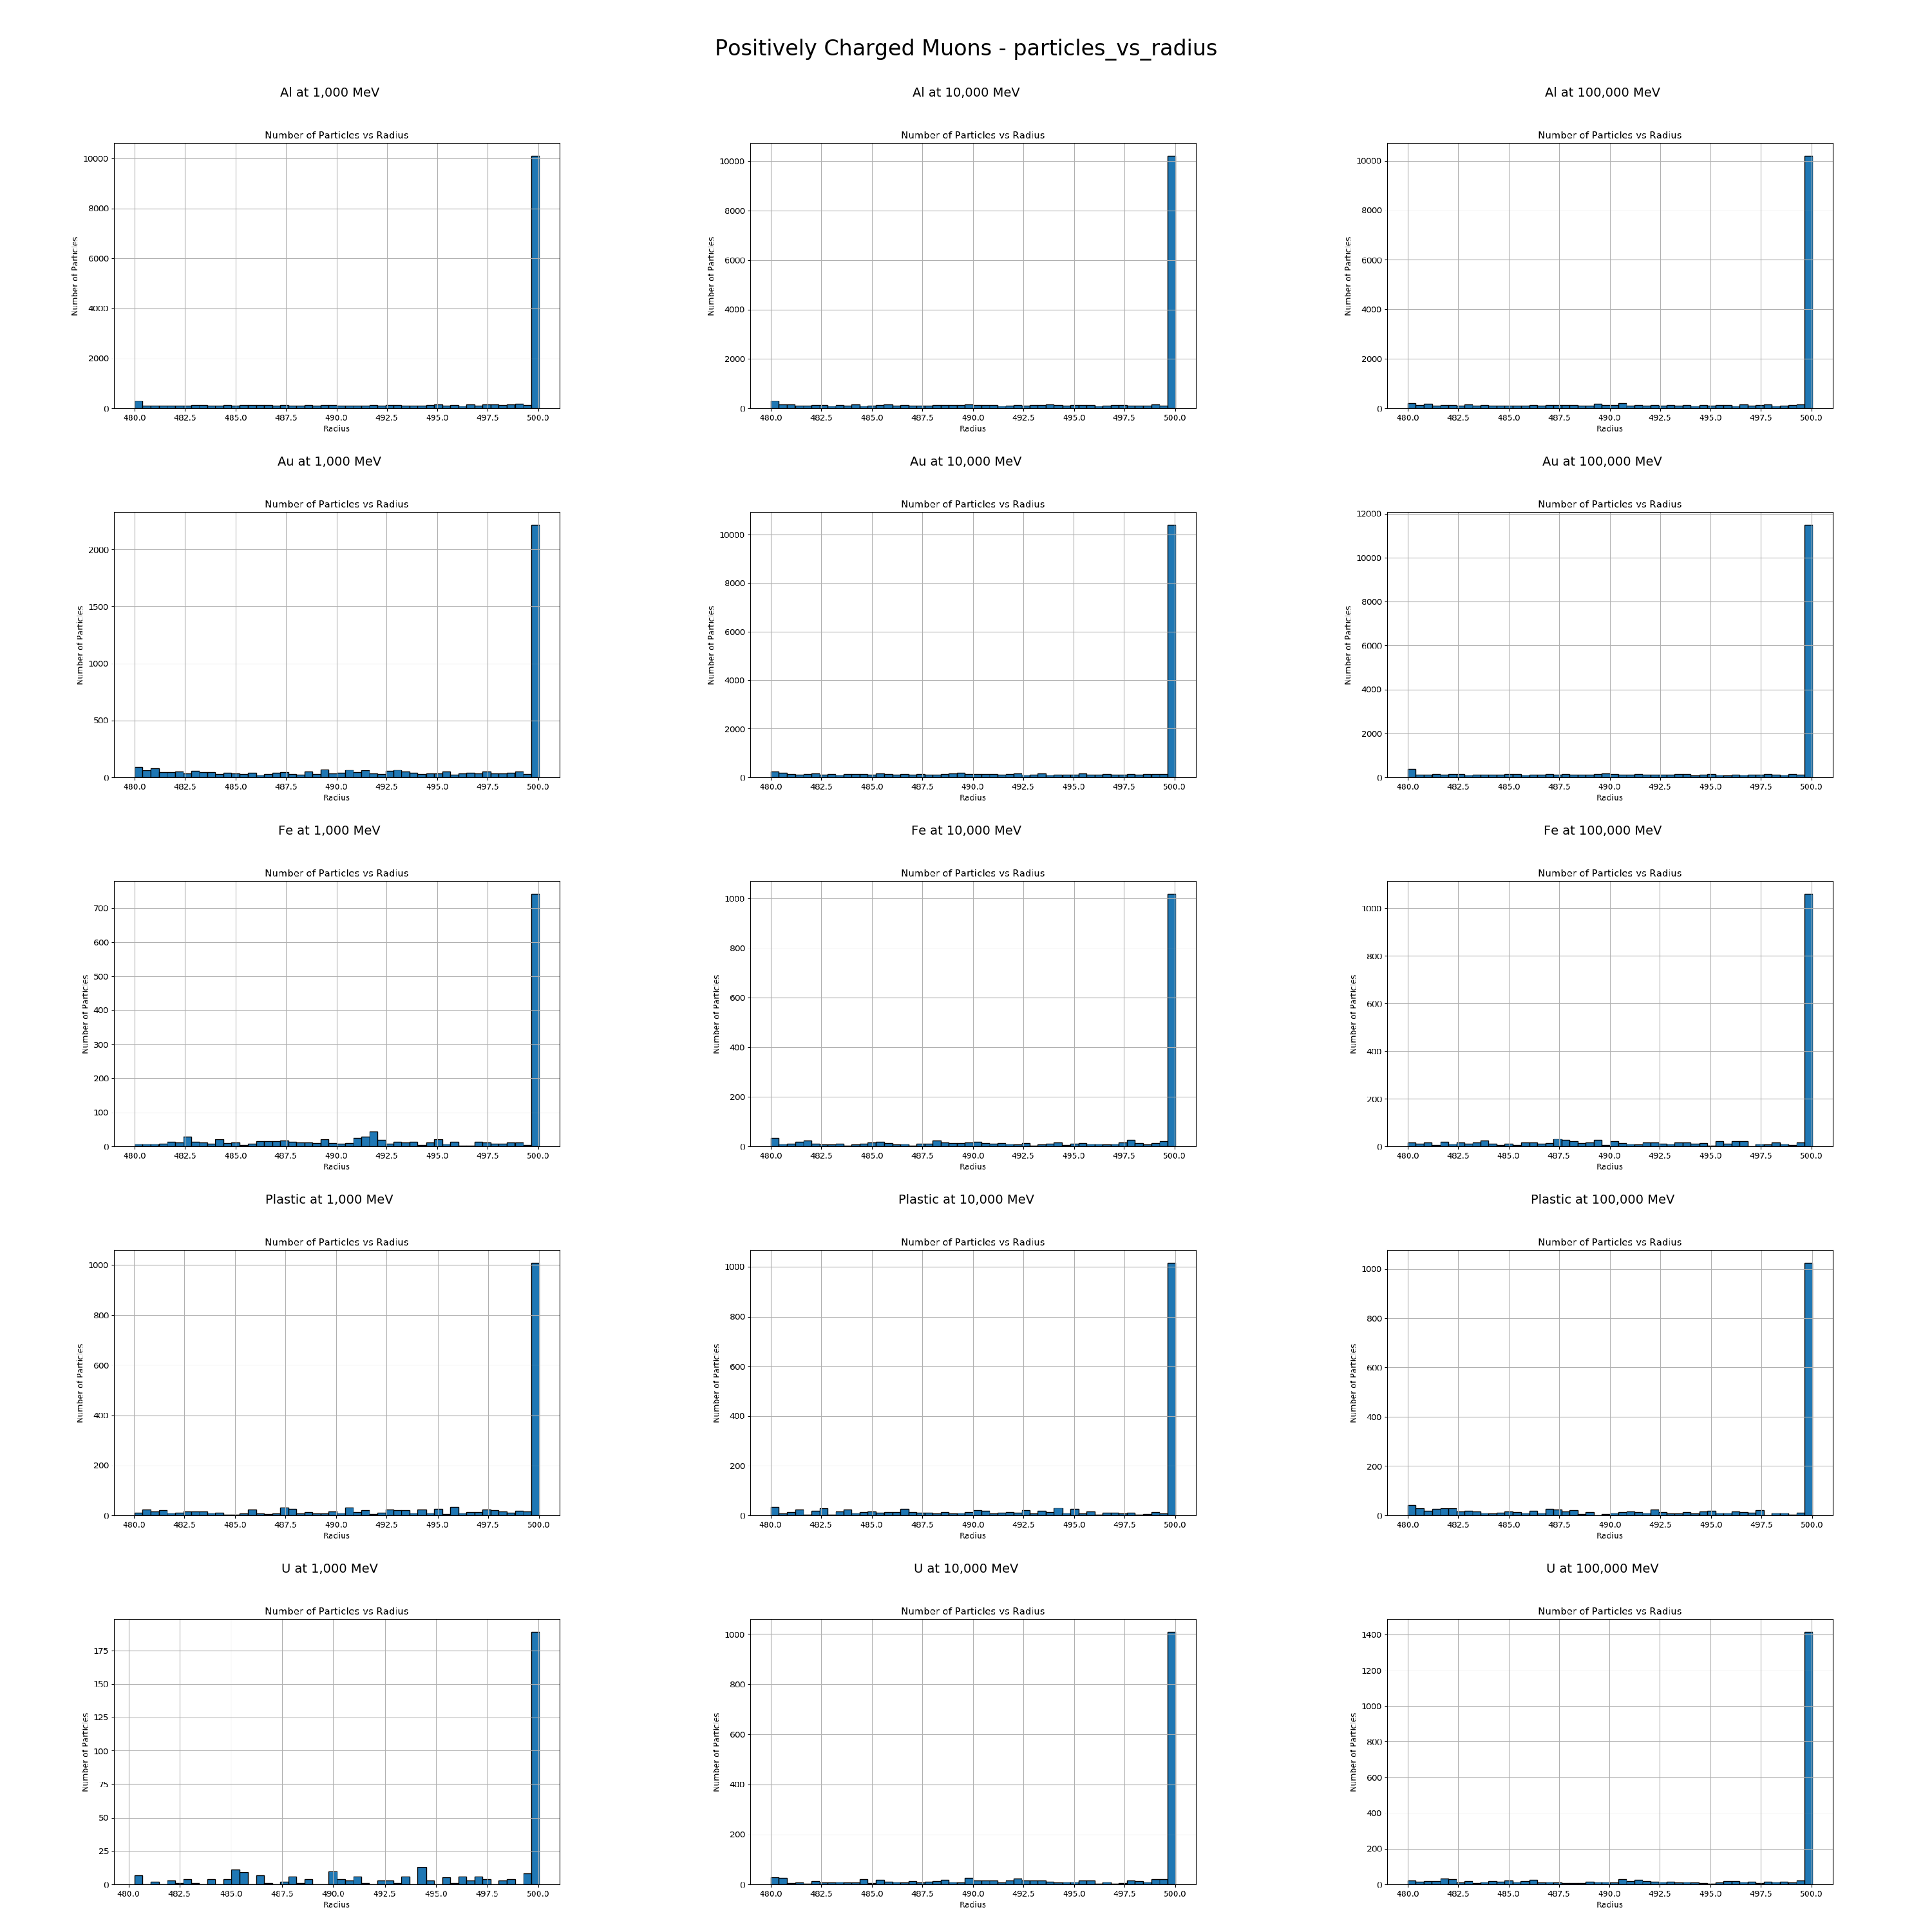
\includegraphics[width=\textwidth]{Combined Plots/particles_vs_radius_mu+.png}
            \footnotesize{Constant for 10,000 and 100,000 MeV, but really depends on what material you are using for 1,000 MeV.}
        \end{figure}
    \end{minipage}
\end{itemize}
\end{frame}

%------------------------------------------------

\begin{frame}
\frametitle{Negatively Charged Electrons (mu-) - \# of Particles vs Radius of Detector Plane}
\begin{itemize}
    \item 
    \begin{minipage}{0.5\textwidth}
        \begin{figure}
            \centering
            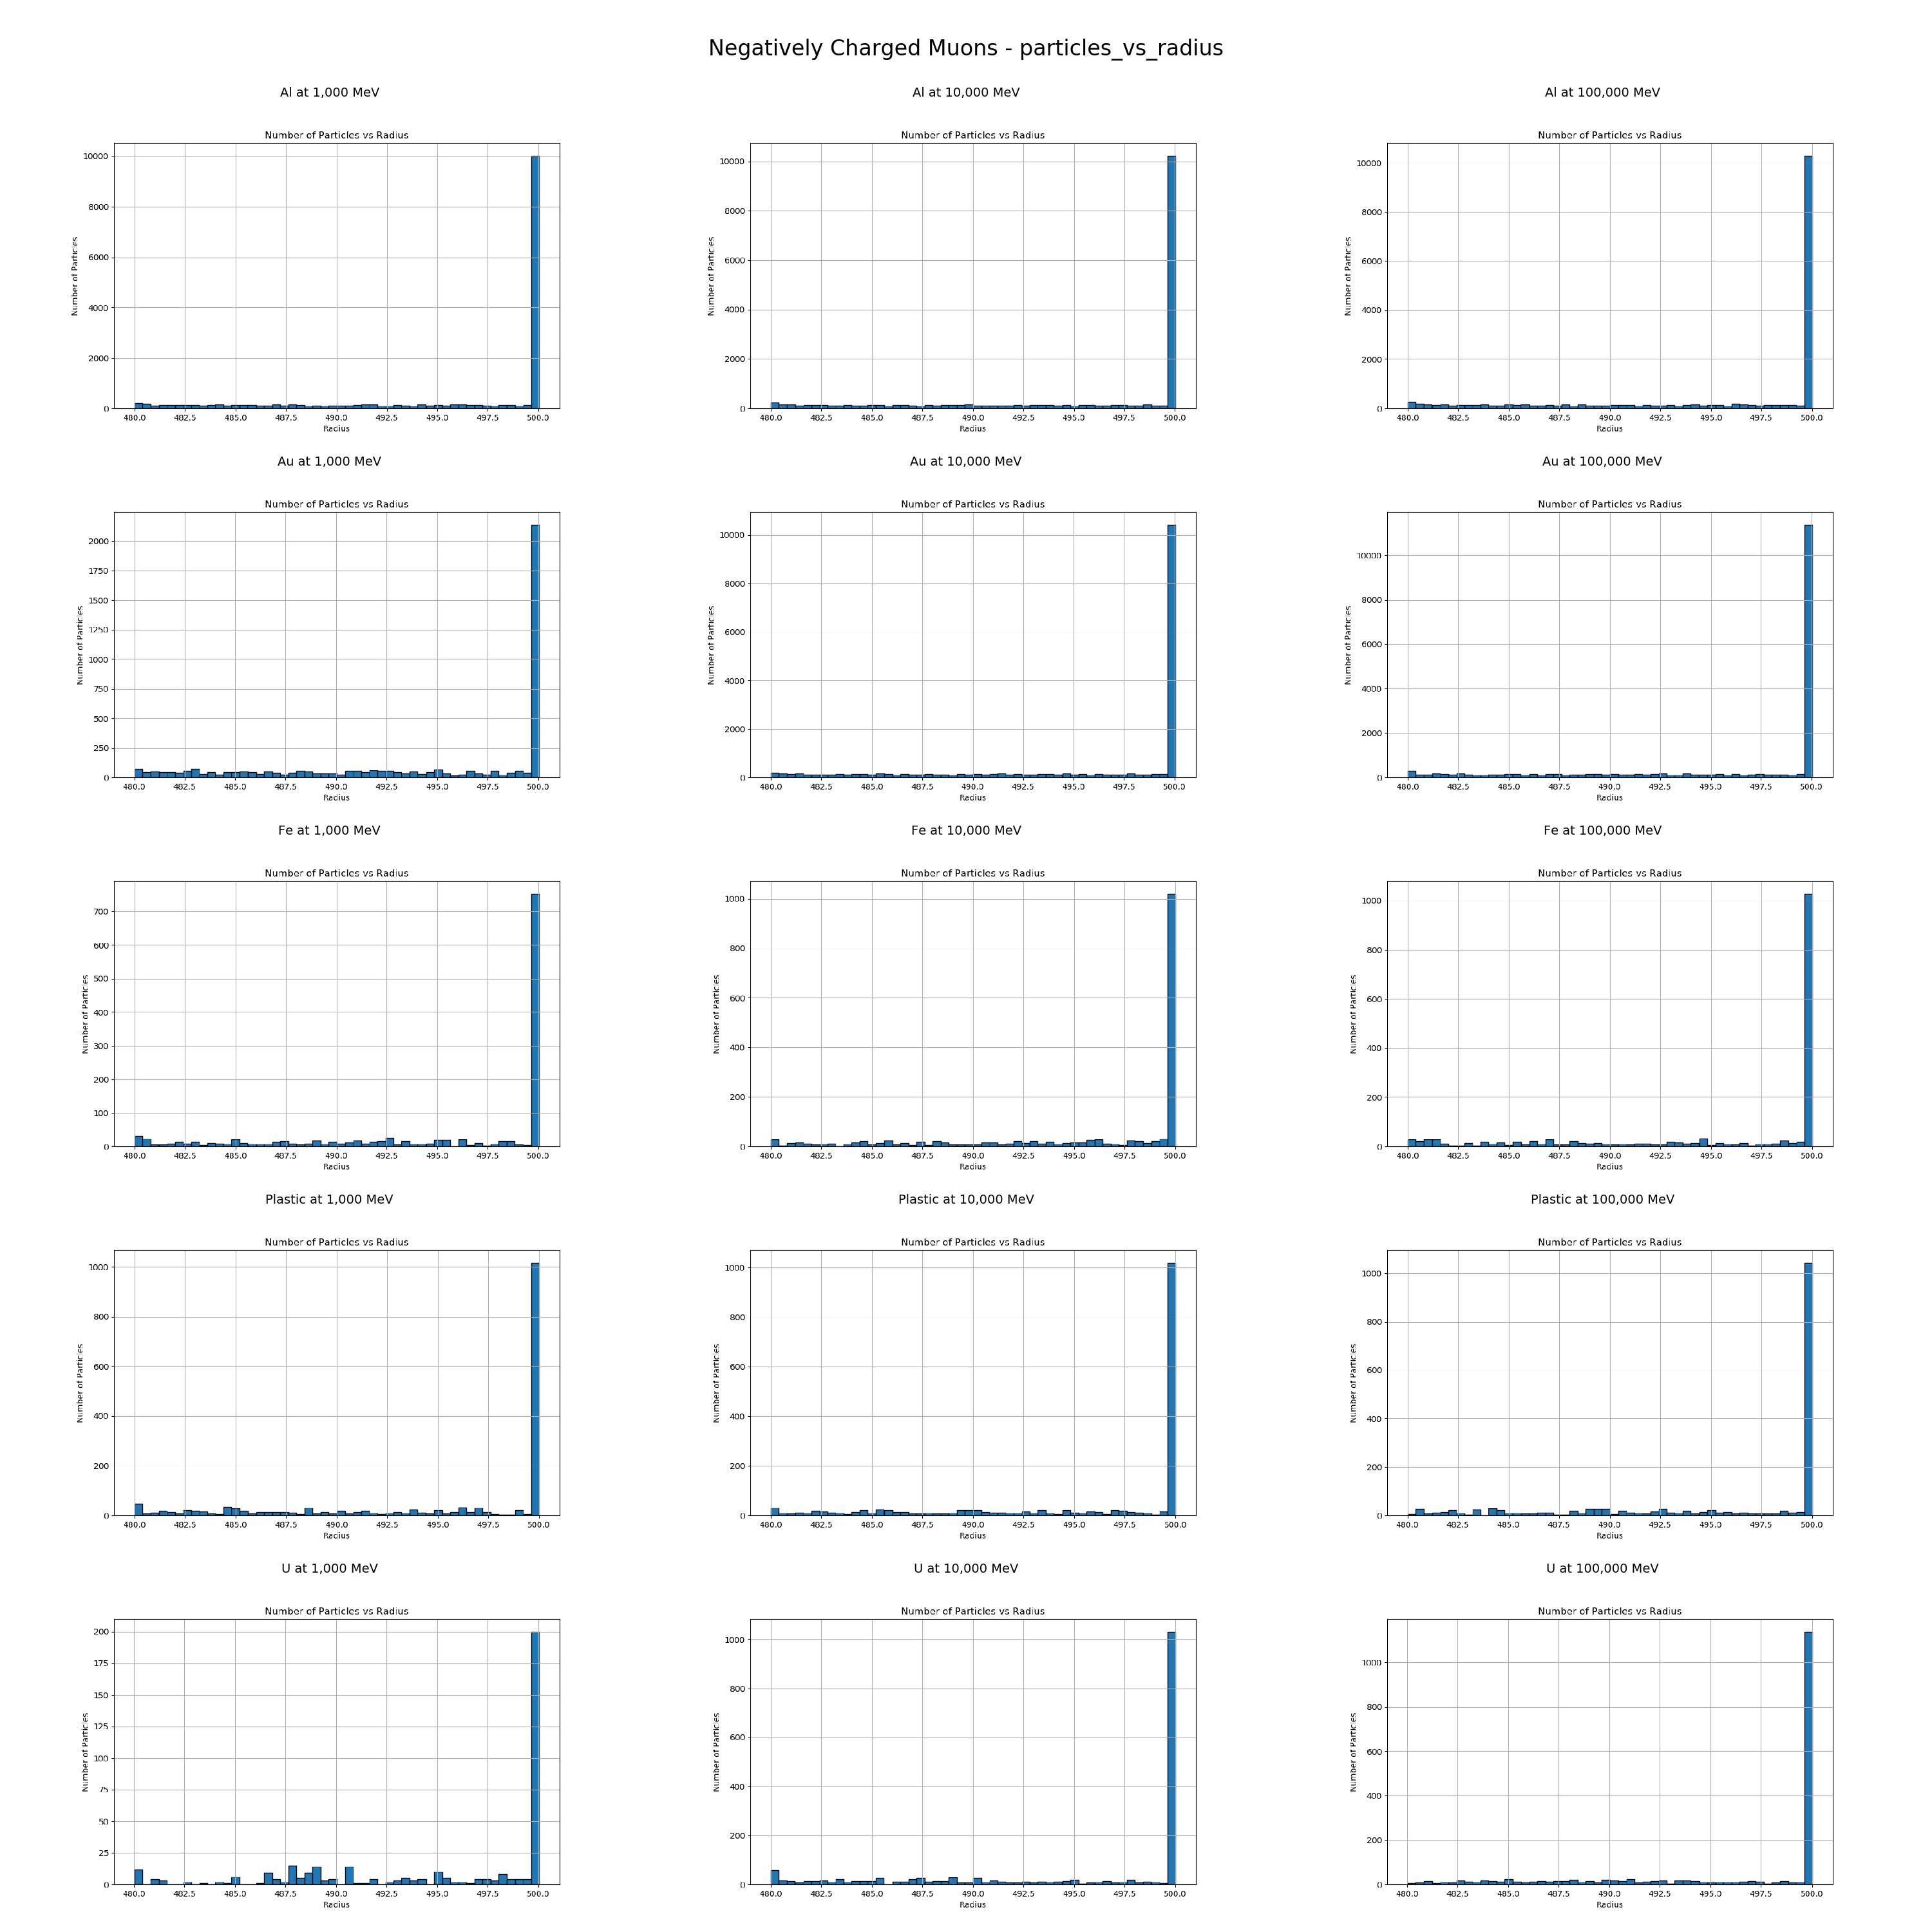
\includegraphics[width=\textwidth]{Combined Plots/particles_vs_radius_mu-.png}
            \footnotesize{Same idea as previous one.}
        \end{figure}
    \end{minipage}
\end{itemize}
\end{frame}

%------------------------------------------------

\begin{frame}
\frametitle{Challenges}
\begin{itemize}
\item Not much documentation
\item Didn't enable Multi-thread Mode
\item Extracting data from simulation
\end{itemize}
\end{frame}

%------------------------------------------------

\begin{frame}
\frametitle{Future Work}
\begin{itemize}
\item Run it on Multi-threading mode
\item More quantitative data analysis
\item More volumes
\item Try more materials, particles, and energy levels
\end{itemize}
\end{frame}

%----------------------------------------------------------------------------------------

\end{document}